\chapter{Fundamental Concepts}\label{ch:fundamental_concepts}
%%%%%%%%%%%%
%- Short introduction what we will go over.
%%%%%%%%%%%%
This chapter tries to condense the theoretic concepts that will reoccur throughout the present thesis. We start off in section \ref{sec:xfel} with an introduction to the key aspects of X-ray free electron lasers (XFEL) including the beam operating modes self-amplified spontaneous emission (SASE), self-seeding and X-ray pump -- X-ray probe. Section \ref{sec:cluster-theory} is about the formation of rare gas clusters via supersonic jets and pickup sources. We then dive into the interaction of light and matter in section \ref{sec:light-matter-interaction} that discusses coherent, elastic X-ray scattering, and inelastic processes in atoms. The chapter ends with section \ref{sec:ionizatin-of-ext-obj} describing the nanoplasma formation in pristine cluster and core-shell systems.
%
%
%
\section{Why X-ray free electron laser?}\label{sec:xfel}
%%%%%%%%%%%%
%- A historic introduction to FELs\\
%%%%%%%%%%%%
%The advance of X-ray free electron laser in the recent years has enabled experimental ideas from long ago but has also opened entirely new branches to research \cite{Pellegrini-2016-RMP,Bostedt-2016-RMP}. So, let us start by investigating how that is. Thus far mostly synchrotron radiation facilities have provided X-rays to a great variety of scientific communities.
%Electromagnetic radiation or light in the X-ray wavelength regime\footnote{Wavelengths of 0.01 of 10nm.} are world famous for their applications in medicine, where X-ray images\index{X-ray!images} allow a non-invasive look inside the body. X-rays are also heavily used in science, where they are heavily used to reveal structures of very small particles, for example proteins - the workhorse bio-molecule in the human body.
X-rays were first created through \textit{Bremsstrahlung}\index{X-ray!Bremsstrahlung}, where an electron beam with kinetic energies $E_{\text{kin}}$ of 100eV - 100keV hit a block of copper and the deceleration of electrons in the copper led to the creation of X-rays. Since then, there has been tremendous progress in the creation of X-rays and are commonly created in synchrotron facilities for scientific purposes. In a synchrotron facility, electrons are accelerated near the speed of light $E_{\text{kin}}>MeV$ and then injected into a storage ring. The electrons are deflected at bending magnets to circle around the ring. The acceleration at the bending magnet leads to the emission of X-rays. Typically, electrons are bunched together to increase the amount of emitted photons and a synchrotron can store many electron bunches, thus a high repetition rate of light pulses on the order of megahertz. The X-ray pulses are characterized through the so called spectral brightness \cite{Mills-2005-IUCR} or sometimes brilliance\index{brilliance|seealso{spectral brightness}}. We can define the spectral brightness\index{spectral brightness} as \cite{Als-Nielson-2011-JWS}
\begin{equation}
B = \frac{n}{A\ \Theta\ \Delta\! E},
\label{eq:spectral-brightness}
\end{equation}
with $n$ being the number of photons per second, $A$ the source area, $\Theta$ the divergence of the beam, and $\Delta\! E$ 0.1\% of the spectral bandwidth of the light pulse. The spectral brightness is an overall measure of the quality of a light source. The development of modern synchrotron light sources is hence often measured and compared to previous achieved B values. The motivation to improve the spectral brightness is to let a sample interact with as many photons possible, in the shortest time as possible and with an energy resolution as best as possible. In other words, more brilliant light sources are needed to create images of even smaller particles, or investigate dynamics that are even faster.
\begin{figure}[t]
	\centering
		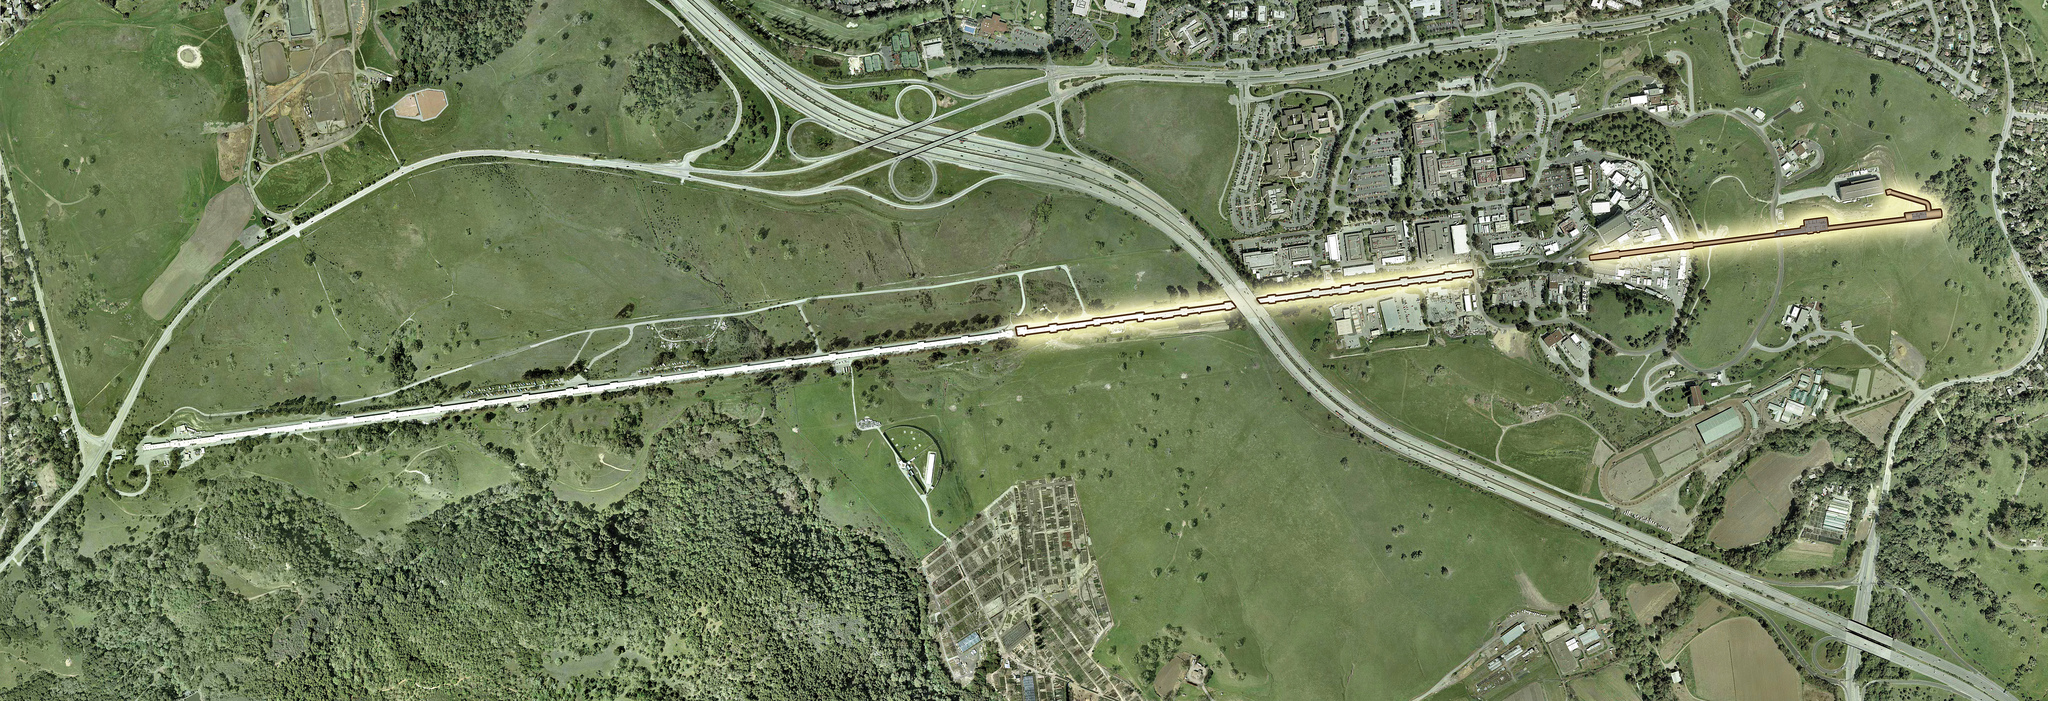
\includegraphics[width=1.00\textwidth]{images/aerial-view-lcls.jpg}
	\caption[Aerial view of the Linac Coherent Light Source.]{Aerial view of the Linac Coherent Light Source\index{Linac Coherent Light Source} (LCLS). LCLS\index{LCLS|seealso {Linac Coherent Light Source}} uses the last third of the SLAC Linear Accelerator but is overall a ~4.1km long machine. The accelerator and buildings are stretched far because of the process light is generated. From \cite{SLAC-2009-Flickr}}
	\label{fig:aerial-view-lcls}
\end{figure}
To give a numerical example and to get a better understanding of the improvements needed, let us look at non-linear absorption dynamics in atoms and molecules. One can conservatively estimate that a typical absorption cross section at soft X-rays\footnote{X-rays with wavelengths of 10nm to 0.2nm.} is around $\sigma = 1$ megabarn (Mb) \cite{Bucksbaum-2011-Book}. Typical X-ray focii are\footnote{Focus size at the AMO endstation at LCLS.} $A = 1 \mathrm{\mu m}^{2}$ such that the number of photons $n_{in}$ needed to absorb just 1 photon per atom $n_{abs}$ is
\begin{equation}
n_{in} = \frac{n_{abs} A}{\sigma} = \frac{10^{-8} \mathrm{cm}^{2}}{10^{-18} \mathrm{cm}^{2}}=10^{10}\qquad \mathrm{photons.}
\label{eq:absorption-cross-section}
\end{equation}
An example of a modern synchrotron source is NSLS-II and it produces $1.7 10^{4}$ photons per pulse in the Si111 bandwidth at pulse durations of a few ten picoseconds \cite{Williams-2016-PC}. That is far out of reach to investigate non-linear, or multi-photon, processes. While this back on the envelope type of calculation might be off by an order of magnitude or so depending on the specific case, it illustrates the order of magnitude improvement scientists were looking for to unravel entire new aspects of nature. As it is not possible to use conventional optical methods to control X-rays, a progressive United States defense program in the 80's ignited an atomic bomb to create an X-ray beam that was intended for use as anti-(space)missile defense \cite{Hecht-2008-OPN}. In a similar time, it was also proposed to build free electron laser \cite{Kondratenko-1980-PA,Bonifacio-1984-OC} to increase the spectral brightness.
Free electron laser, amplify the light along a straight line to create optical laser alike radiation and a FEL can be seen in birds eye view in figure \ref{fig:aerial-view-lcls}. Construction of the first hard X-ray finished in 2009 and the FEL is called Linac Coherent Light Source (LCLS)\index{Linac Coherent Light Source}. X-ray free-electron lasers (XFEL) are able to create $10^12$ photons per pulse and achieve pulse lengths of a few femtoseconds and allow the study of ultrafast processes, for example the movement of electrons in chemical reactions \citep{Emma-2010-NatPho,Young-2010-Nature}. The beam parameters of FEL increased the spectral brightness by many orders of magnitudes\footnote{See figure \ref{fig:soft-xray-self-seeding} for an illustration of the improvement in brilliance.} and we will explore this topic in detail in the next few subsections. Few XFEL exist today, LCLS at SLAC National Accelerator Laboratory in the United States, SACLA at RIKEN in Japan but more are being build. The European XFEL near DESY\footnote{abbreviation for Deutsches Elektron Synchrotron} in Germany, the SwissFEL at Paul Scherrer Institut and the PAL-XFEL at Pohang Accelerator Laboratory in South Korea.
%While some applications are still under development \cite{Aquila-2015-StrucDyn,Weninger-2013-PRL}, free electron laser have made it possible to screen smaller protein crystals then previously possible to measure \cite{Chapman-2011-Nature} and are on track to study the thus far unknown protein structures \cite{Barends-2014-Nature}.
\subsection{From bending magnets to undulator}\label{sec:undulator}
%%%%%%%%%
%- Idea and schematic setup\\
%- Explain SASE including micro-bunching\\
%- Talk about the importance of monitoring the energy loss
%%%%%%%%%
\begin{figure}[t]
	\centering
		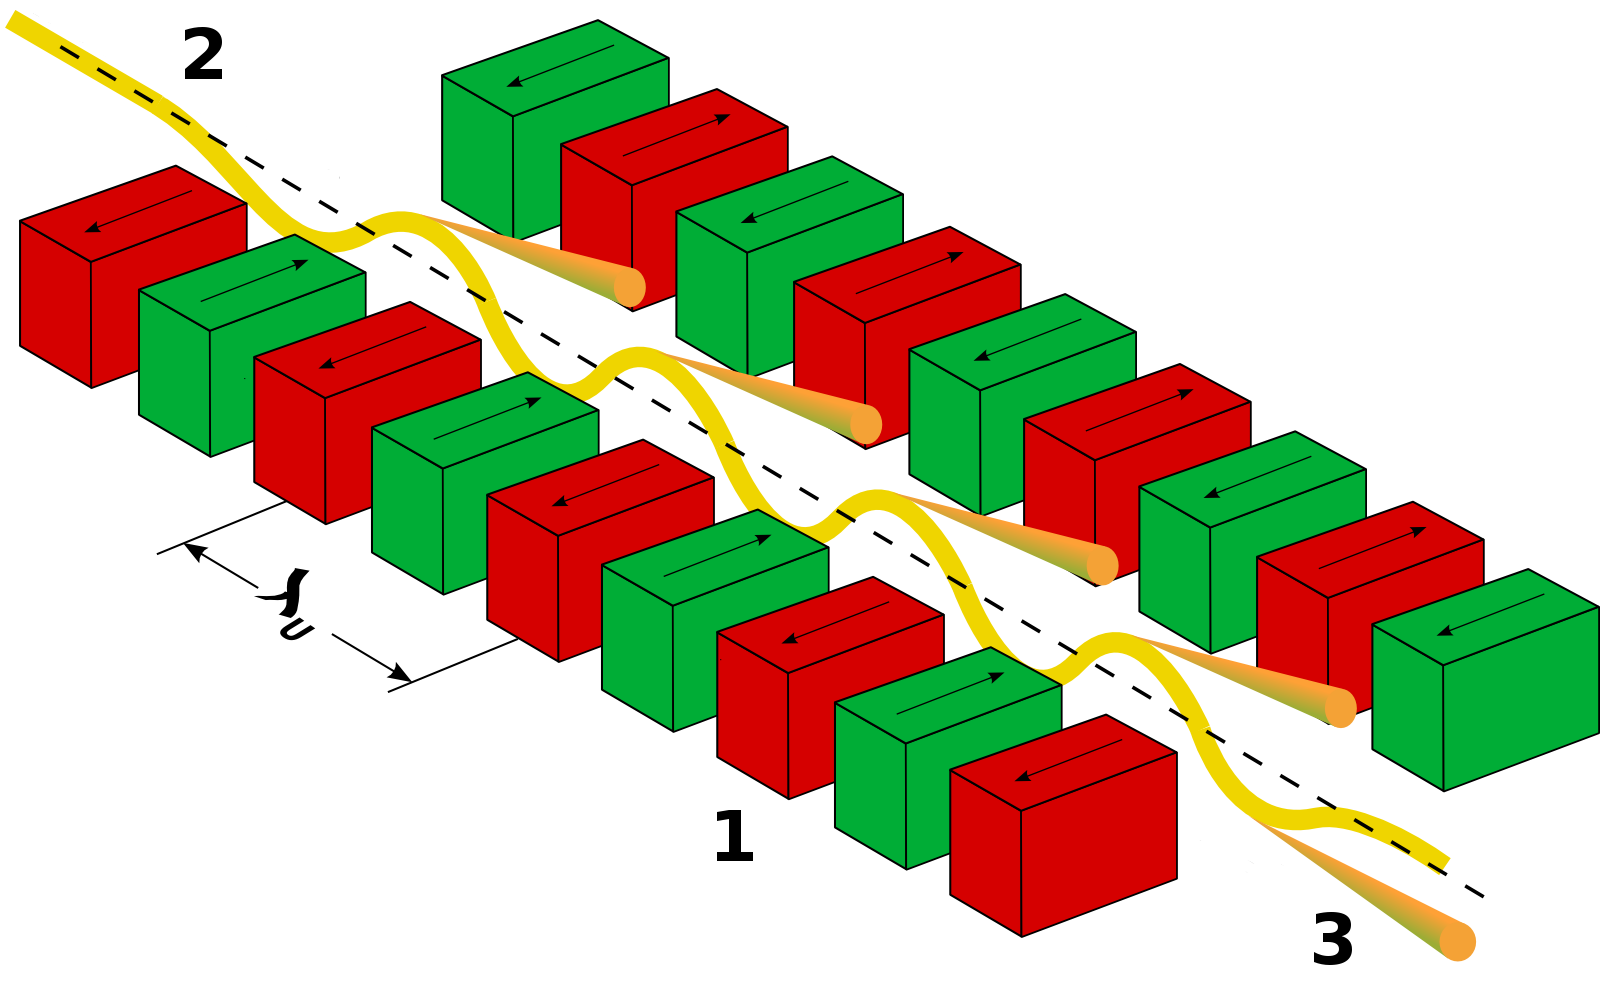
\includegraphics[width=1.00\textwidth]{images/Undulator.png}
	\caption[Schematic setup of an undulator.]{Schematic setup of an undulator with a period of $\lambda_{U}$. (1) Magnets in alternating polarity; the arrows indicate the direction of the magnetic field. (2) Incoming electron bunch near the speed of light. (3) Emitted light in beam direction due to sinusodial movement of the electron bunch. From \cite{holst-2005-wiki}.}
	\label{fig:undulator}
\end{figure}
In synchrotron lightsources as well as free electron lasers, X-rays are generated using (bending) magnets. The first improvement to creating X-rays at a bending magnet was through a \textit{wiggler}\index{wiggler}. Wigglers consist of magnets that are arranged in an alternating order to force the electron bunch on a sinusoidal trajectory. An electron bunch that is traveling through a wiggler near the speed of light is wiggled along its path using magnetic fields, which causes the particles to emit radiation. Wigglers can be considered as a series of bending magnets, which is why the total emitted power $P_{emitted}$ is proportional to the number of magnets $m$ \citep{Brown-1983-NIMPR}
\begin{equation}
P_{emitted} \propto m,\quad \mathrm{in\ a\ wiggler\ magnet}.
\end{equation}
The emitted radiation has a broad, continuous spectrum and the center of that spectrum can be controlled by changing the speed or kinetic energy of the electron bunch. Wigglers have been used at the Stanford Synchrotron Radiation Lightsource (SSRL) in 1979 to generate X-rays. Independently from wigglers, undulators\index{undulator} were developed \citep{Williams-2009-xb}. A schematic setup of an undulator can be seen in figure \ref{fig:undulator}. Wigglers and undulators create radiation because of the same principle, an electron bunch is accelerated near the speed of light and then forced on a sinusoidal pathway. In undulators, the separation of magnets is named undulator period $\lambda_{U}$. The undulator period and magnetic fields are chosen such that the emitted radiation per period constructively interferes with each other. Thus the emitted power $P_{W}$ now scales with \citep{Kim-1986-NIMPRA}
\begin{equation}
P_{\text{emitted}}\propto m^{2},\quad \mathrm{in\ an\ undulator\ magnet}
\end{equation}
The emitted wavelengths of undulators have a more narrow spectrum and a higher flux than wigglers. We can further characterize undulator (and wiggler) by the strength parameter $K$, which is given by \citep{Huang-2007-PRSTAB}
\begin{align}
K &= \frac{e\ B_{\text{max}}\ \lambda_{U}}{2 \pi\ m_{e}\ c},
\intertext{with $e$ being the elementary charge, $B_{\text{max}}$ being the maximum magnetic field in the undulator (wiggler), $m_{e}$ being the mass of an electron and $c$ being the speed of light, we can write in convenient units}
K &\approx 0.934 B_{max}\ \lambda_{U}\qquad \left[\mathrm{T\ cm}\right].
\label{eqn:undulator-strength}
\end{align}
Undulator typically have $K<1$ Tcm (and wiggler $K\gg1$ Tcm). Undulator magnets are large constructs of a few meters and their undulator period is on the order of centimeter. The electrons emit radiation in the nanometer wavelength regime because the electrons near the speed of light have to be considered relativistic and in view of the electrons the undulator period $\lambda_{U}$ appears shorter. We can account for the relativistic effects and express the resonantly amplified wavelength $\lambda_{r}$ by \citep{Huang-2007-PRSTAB}
\begin{equation}
\lambda_{r} = \frac{\lambda_{U}}{2 \gamma}\left(1+\frac{K^{2}}{2}+\gamma^{2}\Psi^{2}\right),\label{eqn:fundamental-wavelength}
\end{equation}
with the kinetic energy $\gamma$ of the electron bunch in the undulator and the electrons observation angle $\Psi$. Summarizing, modern lightsources use undulators to generate radiation as these magnets create more photons that have a narrow spectral bandwidth compared to bending magnets and wiggler. Undulators are characterized by the strength parameter given in equation \ref{eqn:undulator-strength}, which is only dependent on the undulator gap $\lambda_{U}$ and the magnetic field $B$. The fundamental amplified wavelength is given by the resonance condition equation \ref{eqn:fundamental-wavelength}.\\
\begin{figure}
	\centering
		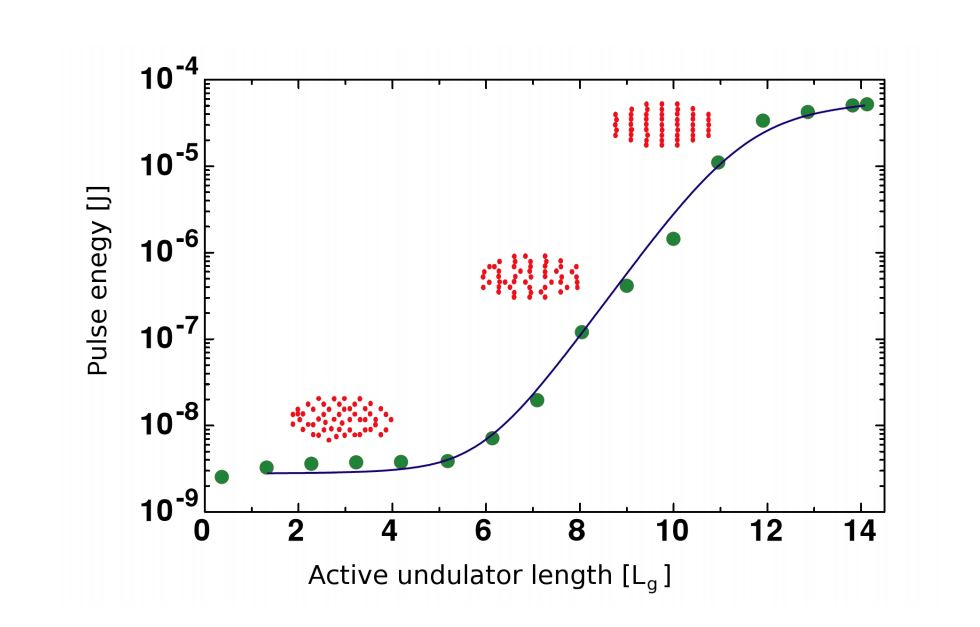
\includegraphics[width=1.00\textwidth]{images/gain-length.JPG}
	\caption[Undulator gain curve correlated to microbunching.]{Undulator gain curve correlated to microbunching. The X-ray pulse energy is plotted algorithmically over the undulator length $L_{g}$ (blue curve, green dots) and shows an exponential growth until saturation. The electron bunch (red dots) is starts with a random density distribution, as the bunch travels through the undulator modulates the electron density and the electrons are microbunched. Upon optimal microbunching, the X-ray lasing process saturates. From \citep{Rupp-2013-Thesis,Rupp-2016-Springer}}
	\label{fig:gain-length}
\end{figure}
\subsection{Self amplification by spontaneous emission}\label{sec:sase}
If an electron bunch travels through just one undulator, the emitted power scales with linearly with the number of electrons $N_{e}$, which is due to the finite size and random electron density distribution of an electron bunch. If the electrons emit light from the same point or separated by $n\ \lambda_{r}$ $\left(n=\left\{1,2,3,...\right\}\right)$ the emitted photons would constructively interfere and would be coherent. FEL use this idea to generate their light pulses. FEL have a straight and long undulator section\footnote{LCLS has a 112m long undulator section.}, where multiple undulators are connected in series. As the electron bunch travels through the FEL undulator section, microscopic effects play a role that could be neglected in typical synchrotron radiation sources. In vacuum, light will always be faster than electrons near the speed of light. This slight velocity difference means that the co-propagating photons and electrons have a phase difference and interact with each other. Depending on the phase, an electron will either gain or loose velocity. Over each undulator period, we can describe this \textit{slippage}\index{slippage} with $\lambda_{r}(\Psi = 0)$. As a result, the initial uniform electron density is periodically modulated. The modulated electron bunch structure is called \textit{microbunching}\index{microbunching}. The creation of micobunching as it travels through undulators is illustrated in figure \ref{fig:gain-length}. The increasingly structured electron beam amplifies a more narrow wavelength bandwidth and the number of electrons that are in phase with the photons increases over the travel length through the undulator. The lasing process saturates when the microbunching is fully developed. Initially (random) created photons in the undulator define the microbunching as it travels through the undulators and amplifies these photons through subsequent spontaneous emission. Hence, this type of radiation (or FEL operation mode) is called \textit{Self Amplification by Spontaneous Emission} (SASE). SASE achieves laser alike amplification of the radiation power $P_{SASE}$ scales \citep[see][p.~61]{Als-Nielson-2011-JWS}
\begin{equation}
P_{SASE} \propto N_{e}^{2},\quad \mathrm{SASE\ operation}
\end{equation}
SASE spectra can be seen in figure \ref{fig:SASE-spectra}. A SASE spectrum is different from shot-to-shot and has distinct peaks that are defined by the initial photons on top of a more broad background.
\begin{figure}
	\centering
		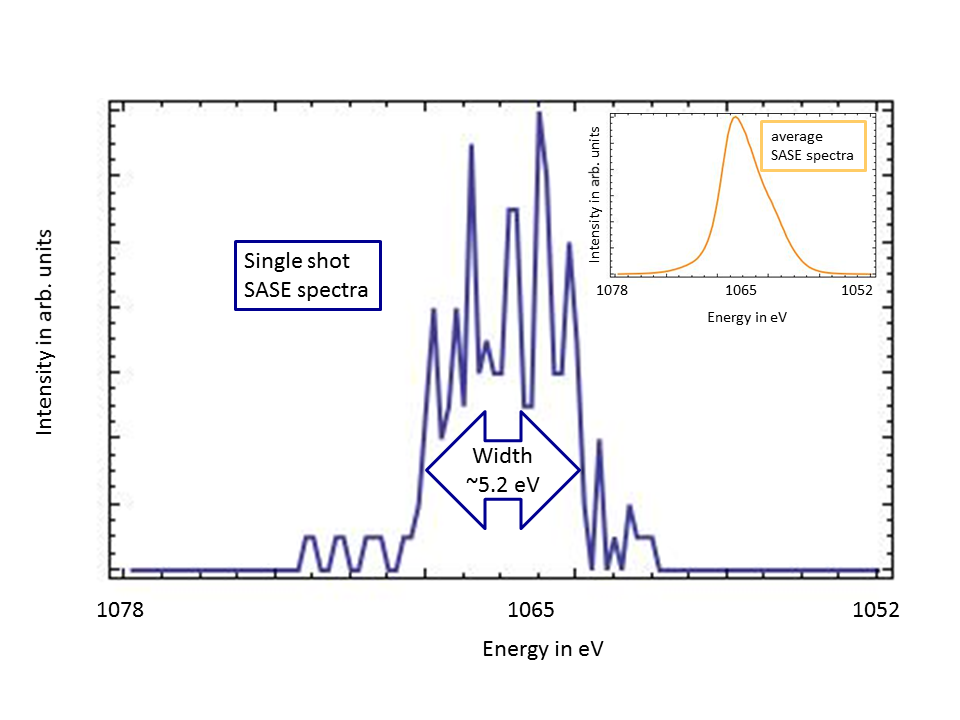
\includegraphics[width=1.00\textwidth]{images/SASE-spectra.png}
	\caption[SASE single-shot and average spectra]{Spectra of FEL SASE operation. The large blue spectra is a SASE spectra from a single FEL shot using a photoelectron spectrometer as described in \citep{Bucher-2014-Unpublished}. Note the spiky peak structure on a background pedestal. Within the narrow bandwidth of a FEL pulse some energies are getting more strongly amplified due to the microbunching. The yellow graph in the inset is an average spectrum of several hundred single-shots and has a low energy tail, which is due to FEL-jitter.}
	\label{fig:SASE-spectra}
\end{figure}
The electrons interact with the light field because of their narrow spatial and kinetic energy distributions that define the so called \textit{emittance}\index{emittance} of an electron bunch. Only the linear accelerator of FEL are able to compress an electron bunch in space and energy, i.e. create a low emittance electron bunch, such that it can interact with the photons and microbunch. Since the creation of X-rays affects the kinetic energy of the electron bunch $\gamma$ and the lack of optics, XFEL use one (compressed) electron bunch\footnote{the European XFEL uses a so called bunch train, where multiple electron bunches are accelerated in series.} in a long set of undulators to create one light pulse. This is also called a \textit{single-pass high-gain} FEL. Without going into much detail, optics can be used to build \textit{multi-pass low-gain} FEL that are able to reuse electron bunches \citep{Kim-2008-PRL}, which leads to higher repetition rates and more narrow spectrum but fewer photons per pulse.
%
%
%
%
\subsection{Soft X-ray self seeding}
%%%%%%%%%%%%%%%%%%%%%%
%- Should I include this section? I could use it for the pump probe as well\\
%- Self seeding vs. seeded FELs\\
%- Schematic setup of a self seeding unit\\
%- Work towards self-seeded beams including spectrometer data
%%%%%%%%%%%%%%%%%%%%%%
\begin{figure}
	\centering
		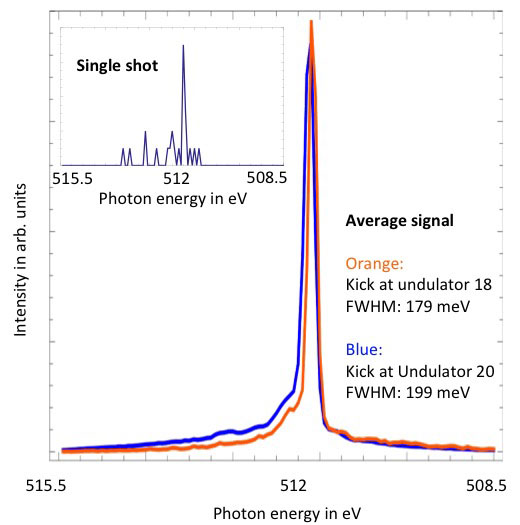
\includegraphics[width=0.49\textwidth]{images/Soft-X-ray-self-seeding.jpg}
		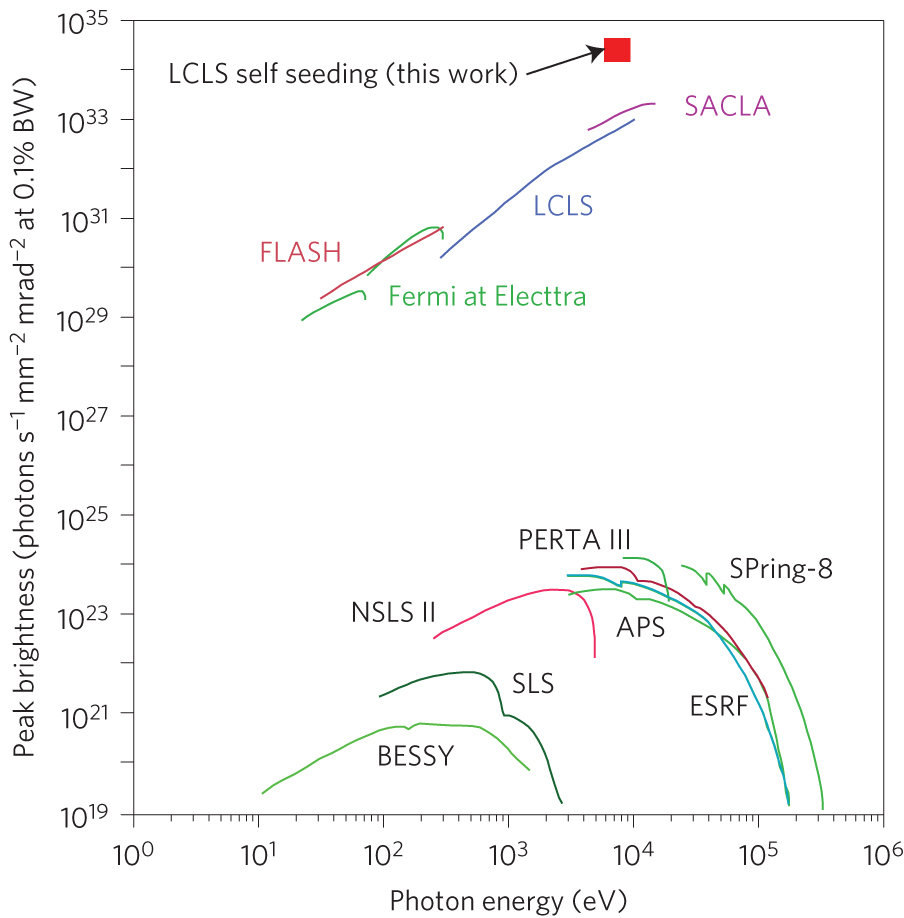
\includegraphics[width=0.49\textwidth]{images/spectral-brightness-fletcher-2015.jpg}
	\caption[Soft X-ray self-seeding spectra and brilliance of various lightsources.]{Left, normalized average spectra of soft X-ray self-seeding operations using the SXRSS and AMO instrument at LCLS \cite{Bucher-2014-Unpublished}. The self-seeding spectra is characterized by a sharp spectral peak around a desired energy accompanied by a SASE radiation type spectral pedestal. The often undesired SASE pedestal is suppressed, when the electron bunch travel through undulators is shortened, here kick at LCLS undulator 18 vs. 20. The right image shows the peak spectral brightness of various light sources over a wide photon energy range. Soft X-ray self-seeding has a spectral brightness that exceeds current SASE FEL sources. From \citep{Fletcher-2015-NatPho}.}
	\label{fig:soft-xray-self-seeding}
\end{figure}
Another FEL beam mode is the seeded type. In contrast to the SASE operation, where the inital photons are randomly emitted and further amplfied, a seeded FEL starts with a given \textit{seed} of photons. If the set of inital photons is monochromatic, mostly this wavelength is amplified as the bunch travel through the undulator. The initial photon seed can be created through various processes and the wavelength of the photon seed is the critical parameter in determining which method to choose. For example, in the infra red (IR) to extreme ultra violet (XUV) regime, conventional lasers can be used to place the initial photons seed. However, due to the lack of lasers available at X-rays wavelength regimes, the idea of \textit{self-seeding}\index{self-seeding} gained traction. In self-seeding, an electron bunch is first send through a few undulator magnets to generate a few SASE photons, the electrons and photons are then separated using a magnetic chicane, which also neutralizes the microbunching in the electron bunch. The monochromator selects a small wavelength slice from the comparably broad SASE spectrum of the initial photons. Photons exiting the monochromator are considered as \textit{seed}. The seed and the electron bunch are overlapped again using the magnetic chicane and then send through more undulators. Here, the seed modulates the electron bunch and thus only a narrow spectral band is amplified. A typical spectrum of a soft X-ray self-seeded beam can be seen in the left figure \ref{fig:soft-xray-self-seeding}. The characteristics of a self-seeded spectrum are an intense peak at the selected wavelength regime on top of a broad SASE background pedestal. The background is an artifact of the amplification of some spontaneous emission events and can be suppressed by using fewer undulator magnets. Self-seeded beams have a significantly reduced pulse energy by an order of magnitude, depending on the exact beam parameters, as compared to SASE operations. However, in their main peak, self-seeded beams have a higher spectral brightness when compared to a SASE spectrum. Using equation \ref{eq:spectral-brightness} the increase in spectral brightness compared to SASE is understandable and it is illustrated in the right figure \ref{fig:soft-xray-self-seeding}. Self-seeded beam operations have recently been demonstrated at LCLS. At hard X-rays, the Hard X-Ray Self-Seeding (HXRSS) instrument uses a diamond crystal to select a wavelength slice \citep{Amann-2012-NatPho}. At soft X-rays, the Soft X-ray Self Seeding (SXRSS)\index{self-seeding!soft x-ray} instrument uses a grating as dispersive element \citep{Ratner-2015-PRL}. A seeded beam using an external laser generate photons as initial seed has been demonstrated at the extreme ultra violet (XUV) FEL FERMI at Ellettra-Sincrotrone in Italy \citep{Allaria-2012-NatPho}. The peak intensity in a narrow spectral band makes seeded beams interesting for a variety of applications particular in condensed matter physics, where it is instrumental to excite with narrow bandwidth photons. Of course there are also applications in atomic and molecular physics, ranging from linear absorption spectroscopy \citep{Ferguson-2014-Unpublished}, to ultrafast photoemission spectroscopy on molecules \citep{Bucher-2014-Unpublished}, to non-linear stimulated Raman spectroscopy \citep{Kimberg-2016-FD}, to ultra-fast photoemission studies. Particular interesting for this work is the magnetic chicane from the SXRSS instrument that has been used as described in the next chapter.
%
%
%
%
\subsection{Novel X-ray pump–probe techniques}
%%%%%%%%%%%%%%%%%
%- Albertos pump-probe version\\
%- Agos two color pump probe version\\
%- Ratners and Agos seeded pump probe version\\
%- Use spectra from single-shot spectrometer
%%%%%%%%%%%%%%%%%%%%%%%%
In order to study X-ray induced phenomenon using X-ray imaging and spectroscopy techniques, as it is discussed in the present work, two X-ray pulses are needed . Here, a pump pulse is used to induce dynamics in the sample system and a probe pulse is used to probe them at a certain time delay $\Delta t$. Pump--probe experiments are commonly used as they allow a precise study of dynamics. The pump pulse gives a very controllable starting point, i.e. time zero in the dynamic process, and the probe pulse can perform a measurement at a later time delay $\Delta t$. Sometimes pump and probe pulse are switched, which is indicated by a negative time delay $\Delta t$, often to verify time zero or to probe the system before any dynamics have occurred.\\
Creating two X-ray flashes to create a pump--probe experiment is a technical challenge and again this challenge is due to the lack of X-ray optics. In order to overcome this challenge, two methods have been proposed. Method one, mirror based beam-split and delay systems \citep{Castagna-2013-JPCS,Murphy-2012-SPIE} that split one pulse into a pump and probe beam and allow the delay of the latter. These systems are typically limited to short times delays, as the optics have to fit into existing setups and have a low transmission of X-rays over the mirrors. Method two, uses accelerator based schemes \citep{Lutman-2013-PRL,Marinelli-2015-NatComm} that manipulate electron bunches to create two X-ray pulses. Limitations arise depending on the scheme, e.g. limited pulse delay $\Delta t$ or pulse energy split through limited electron beam separation or length of magnetic chicane. Both methods have been demonstrated at LCLS and have found use to complement the more widely available optical laser pump -- X-ray probe methods particularly in the chemical sciences \cite{Picon-2016-NatComm,Ferguson-2016-SciAdv,Liekhus-Schmaltz-2015-NatComm}.\\
Another aspect to pump--probe experiments is the tunability of wavelengths in each pulses, for example to resonantly pump and off-resonance probe or vice versa. Equation \eqref{eqn:fundamental-wavelength} indicates which parameters can be tuned to create two pulses of different color. One, the undulator parameter K can be tuned to change the emitted wavelength, or two, the lorentz factor $\gamma$ can be different if there are two electron bunches. A potential third option are variable gap undulators that allow a change of period $\lambda_{U}$. At LCLS $\lambda_{U}$ is fixed but future upgrade plans for LCLS-II include variable gap undulators \citep{Galayda-2014-IPAC}. As the accelerator based X-ray pump -- X-ray probe method, let us describe these schemes in greater detail.
%
%
%
\subsubsection{Undulator parameters $K_{1,2}$ based pump--probe scheme}
\begin{figure}
	\centering
		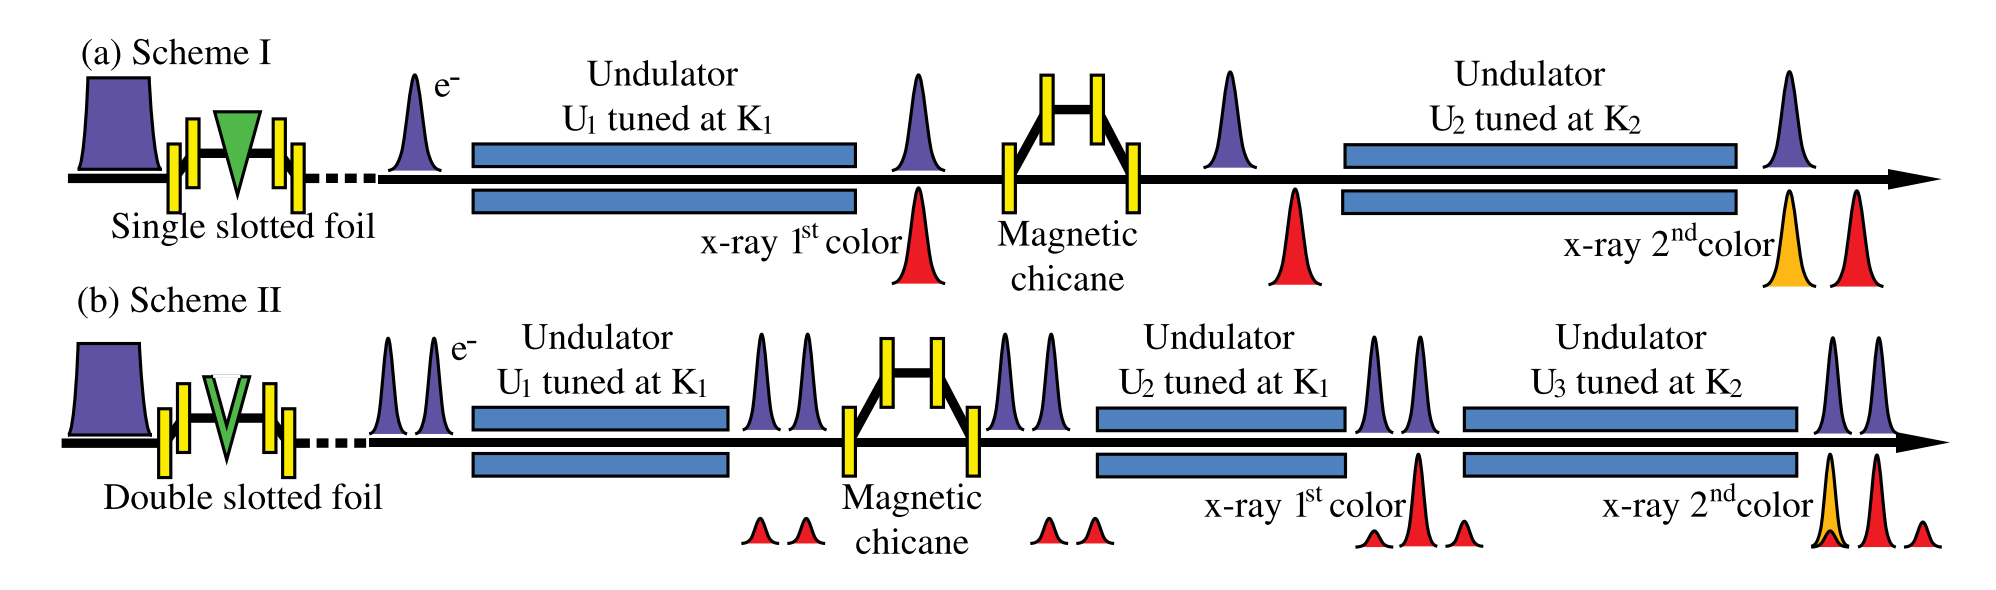
\includegraphics[width=1.00\textwidth]{images/Albertos-pump-probe-scheme.png}
	\caption[Schematic setup of an undulator based pump--probe scheme.]{Schematic setup at LCLS of undulator parameter $K_{i}$ based pump--probe schemes. Scheme I creates one electron bunch using a single slotted foil and scheme II creates two electron bunches using a double slotted foil. The electron bunches emit radiation with a wavelength depending on $K_{i}$. A time delay $\Delta t$ between pulses is introduced using a magnetic chicane. From \cite{Lutman-2013-PRL}. Reprinted with permission from APS.}
	\label{fig:Albertos-pump-probe-scheme}
\end{figure}
The first developed accelerator based pump--probe technique at LCLS \cite{Lutman-2013-PRL} uses a difference in undulator parameters $K_{1,2}$ to create two pulses of different wavelength, the time delay is introduced through a magnetic chicane and a schematic setup can be found in figure \ref{fig:Albertos-pump-probe-scheme}.\\
Following the figure, in scheme I, one electron bunch is created through a single slotted foil\footnote{A single slotted foil or emittance-spoiling foil works comparable to a monochromator. It leaves a certain energy band of the electron bunch within the slot unspoiled and Coulomb scatters or spoils (compare to apertures) the rest. The 'dispersive' element is a magnetic chicane. By narrowing the electron beam one also reduces its pulse duration \cite{Emma-2004-PRL}.}  The use of the slotted foil enables control over the pulse duration. The electron bunch then travels through an undulator section $U_{1}$ tuned at strength parameter $K_{1}$ and is stimulated to lase but the process does not go into saturation such that the electron bunch can be reused in the second undulator section. A magnetic chicane removes the microbunching from section $U_{1}$ such that in undulator section $U_{2}$, tuned to undulator strength parameter $K_{2}$, the electron bunch lases again and the process is able to saturate. The maximal color separation between the two pulses is $~ 1.9\%$ in relative difference between $K_{1}$ and $K_{2}$.\\
The time delay $\Delta t$ between the two pulses is introduced by a magnetic chicane. At LCLS, a dedicated chicane, e.g. from the soft X-ray self-seeding instrument, can reach up to
\begin{equation}
\Delta t_{\text{max}} = 800 fs.
\label{eq:alberto-delta-t-max}
\end{equation}
The minimal time delay can be achieved by setting the deflection in the magnetic chicane to zero in which case
\begin{equation}
\Delta t_{\text{drift}} = \frac{l}{v_{\text{el drift}}} - \frac{l}{c}\approx 0 fs,
\label{eq:alberto-delta-t-min}
\end{equation}
with $l\approx 4m$ being the length between undulator sections $U_{1}$ and $U_{2}$ and $c$ being the speed of light and $v_{\text{el drift}}$ being the drift velocity of the electron bunch. As the electron bunch travels close to the speed of light $t_{\text{min}}$ is typically on the tens of attosecond timescale. The timing jitter between the two light pulses using only one electron bunch comes from the magnetic chicane due to the magnetic field jitter and the electron beam energy jitter. The total contribution to the timing jitter is less than $0.4\%$ of the time delay $\Delta t$ imposed by the chicane. Since the delay chicane does not significantly contribute to the delay $\Delta t_{\text{min}}$ a bigger factor is the velocity mismatch of the light pulse and the electron bunch. This mismatch can be estimated by
\begin{equation}
\Delta t_{\text{min}}-t_{\text{drift}}=\frac{N_{u} \lambda_{r}}{c},
\label{eq:alberto-beam-missmatch}
\end{equation}
with $N_{u}$ being the undulator periods. Given the parameters in study \cite{Lutman-2013-PRL}, $t_{\text{min}}=3fs$ such that a partial overlap between the electron bunch and lightpulse could be achieved after the magnetic chicane. It should be noted that this technique has been used in the described experiment.\\
Scheme II uses a double slotted foil\footnote{A double slotted foil works as a single slotted foil but it leaves to parts of the electron beam unspoiled through the two slots.} to create two electron beams. The two beams have a longitudinal separation that translates into the time delay $\Delta t$. The electron bunches travel through a first set of undulators $U_{1}$ that creates two pulses of the same wavelength, due to the shortness of the section $U_{1}$ the lasing process does not saturate. The electron bunches are then delayed using a magnetic chicane such that the leading electron bunch overlaps with the trailing light pulse. This light pulse now functions as a seed for the leading electron bunch such that this pulse saturates in undulator section $U_{2}$. The electron bunches then travel through the magnets at $U_{3}$, where the trailing electron bunch creates a second saturated pulse, the leading electron bunch barely emits radiation in $U_{3}$ since its energy spread has become too large after lasing in $U_{2}$. Using this method, two saturated lasing pulses can be generated, however, temporal overlap cannot be achieved.
%
%
%
%
\subsubsection{Twin bunch or Lorentz factor $\gamma$ based pump--probe scheme}
\begin{figure}
	\centering
		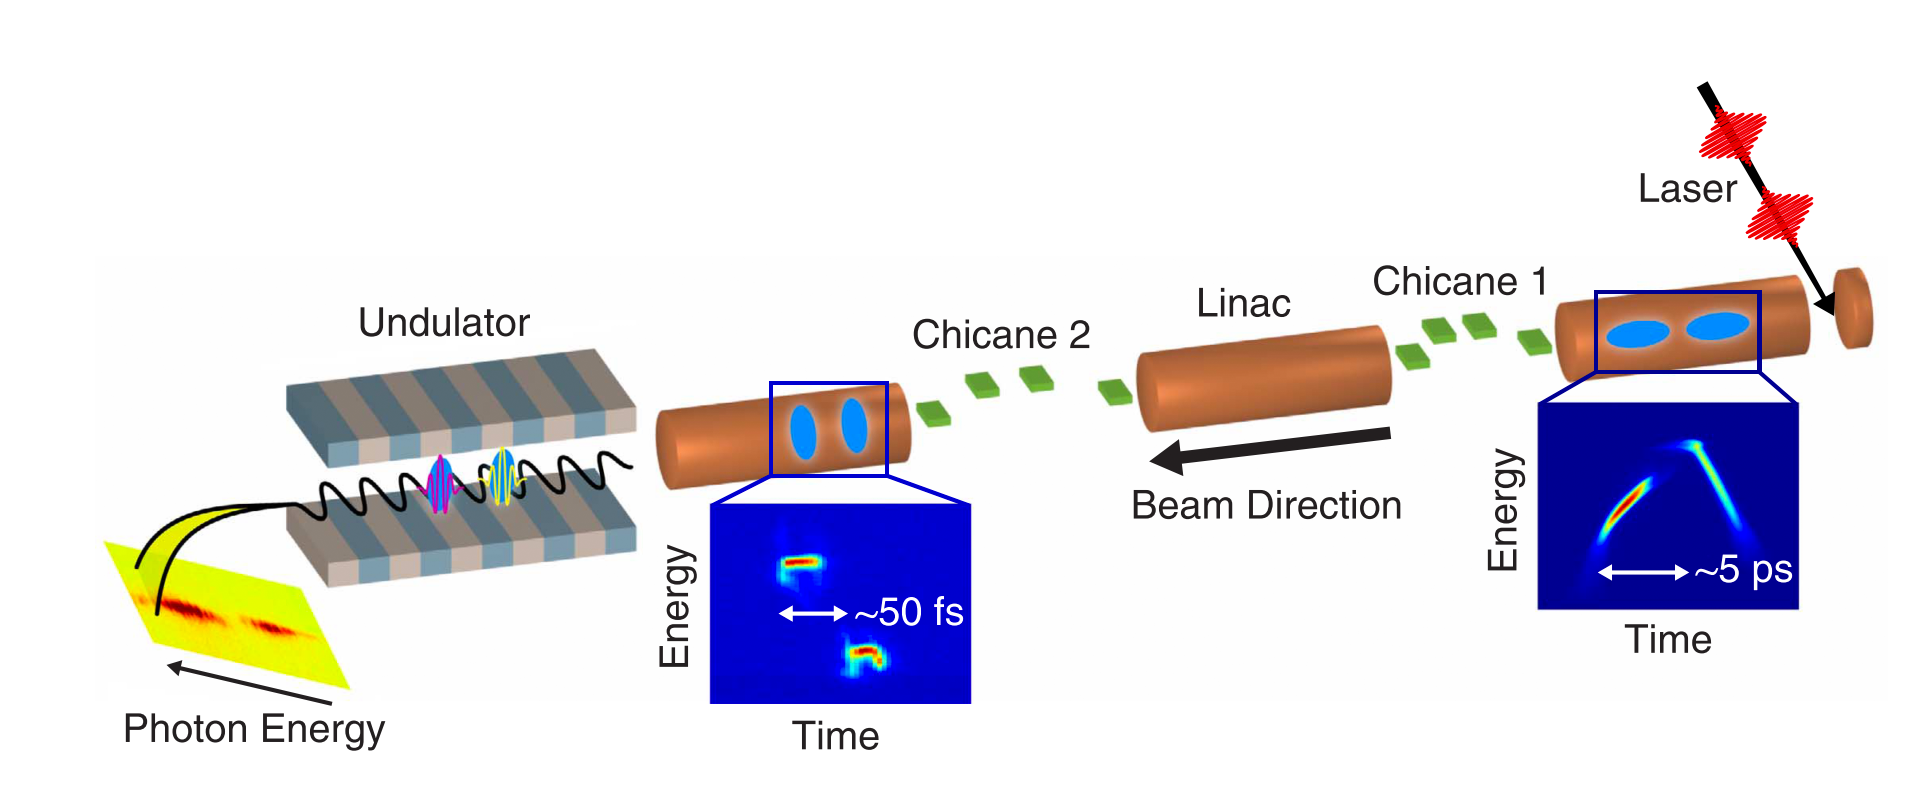
\includegraphics[width=1.00\textwidth]{images/Agos-pump-probe-scheme.png}
	\caption[Schematic setup of a bunch based pump-probe setup.]{Schematic setup of the two bunch, two color pump--probe setup at LCLS. Two laser pulses shot at a cathode create two electron bunches with a delay $\Delta t$ on the picosecond timescale. Two magnetic chicanes compress the bunches such that a delay $\Delta t$ on the up to the ten femtosecond timescale is achieved. Both pulses go through one undulator section and the lasing process is saturated. The relative color separation is on the order of $1\%$ between the bunches. From \citep[\href{http://creativecommons.org/licenses/by/4.0/}{\ccby}]{Marinelli-2015-NatComm}.}
	\label{fig:Agos-pump-probe-scheme}
\end{figure}
The second developed accelerator-based pump-probe technique at LCLS \cite{Marinelli-2015-NatComm} uses two electron bunches of different energy. A schematic setup of this beam operation can be found in figure \ref{fig:Agos-pump-probe-scheme}.\\
The electron bunches are created through a double laser pulse that impinges on a photocathode. Initially, these two bunches have a time delay of a few picoseconds, however, two magnetic chicanes compress the electron bunches in the time and intensity domain such that a time delay on the ten femtosecond timescale is achieved. The electron bunches then travel through one undulator section and both pulses saturate in their lasing process. At $8.3k$ eV, both pulses combined can reach pulse energies of $1.2mJ$, the color separation is $100$ eV and the time separation ranges from $\Delta t_{min}=0fs$ to $\Delta t_{max}=100fs$. At hard X-rays, this method requires the pump pulse to have a higher photon energy than the probe pulse, although their respective intensities may vary. However, this method is not restricted to hard X-rays and can be utilized at soft X-rays. In the soft X-rays wavelength regime, where the slotted spoiler foil can be used. This allows a further control to tune the time delay of the electron bunches and enables scanning across time zero with both pulses.
%%%
\section{Rare gas clusters}\label{sec:cluster-theory}
%%%%%%%%
%- Why are rare gas clusters a suitable sample
%%%%%%%%
Clusters have a long history to study light-matter interaction for a few reasons. Their characteristics are well known, they can form interesting states and often it has practical purposes \cite{Haberland-1994-Springer}. Generally speaking, clusters are an aggregation of atoms or molecules and vary in size. Their size ranges from a few atoms to mesoscopic sizes such that one can classify a cluster as a bulk material. Even though clusters can form exotic materials that are interesting to study, they can be simulated with computer models. Besides these testbed characteristics, clusters can be created comparably easily and are tunable in size. Rare gas clusters are a subclass of clusters and they are bound by van der Waals forces, thus are normally neutral-charged. Single van der Waals cluster typically form in an icosahedral\footnote{An icosahedron is a polyhedron with 20 faces, i.e. a dice with 20 faces.} shape when they are sufficiently small (up to nanometer sized) \cite{Miehle-1989-JCP} and have mostly a fcc-crystal\footnote{fcc is short for face-centered cubic. A very common crystal structure.} structure but exhibit also hcp-crystal\footnote{hcp stands for hexagonal close-packed and is also a crystal structure.} structures \cite{VanDeWaal-1993-JCP,Krainyukova-2006-TSF}. In the present work, superfluid helium cluster (or droplets), solid xenon cluster and a mixture of both have been used as a sample. Therefore, we shall explore the creation of homogenous and heterogeneous rare gas clusters in the next sub-sections.
%
%
%
\subsection{Creation of a homogenous cluster}\label{sec:homogenous-cluster}
%%%%%%
%- the theory behind rare gas cluster creation.
%%%%%%
Rare gas clusters, for example xenon clusters, can be generated in a variety of ways. Often, as in the described experiment, rare-gas clusters are created by releasing gas from a reservoir into a vacuum. Here, a nozzle connects the gas reservoir with the vacuum system and while the gas is expanding through the nozzle, many collisions take place. So, the cluster formation process can be explained intuitively through a kinetic model \cite{Lippmann-1984-JCP}. In other words, clusters grow through collisions with monomer, dimer and other clusters. We can express a collisions mathematically through the following reaction formula
\begin{align}
A_{n}+A_{m} \rightleftharpoons A_{n+m}^{*},\quad n,m=1,2,...,\quad \text{collision,}
\intertext{with $n,m$ denoting the number of monomer assembling body $A_{n,m}$. A body $A_{n}$ collides with another body $A_{m}$ and form a metastable state $A_{n+m}^{*}$ that will dissociate if not a subsequent collision deactivates it}
A_{n+m}^{*}+M\rightleftharpoons A_{n+m} + M,\quad \mathrm{activation/deactivation.}
\label{eq:early-cluster-growth}
\end{align}
$M$ is a chaperone that can be any kind of third body that removes energy from the system. Note that a chaperone $M$ can also activate the state again. The binding force behind rare-gas clusters is the Van der Waals force, hence these clusters are called Van der Waals cluster sometimes.\\
While the early stage of the cluster growth is driven by the monomer addition, cluster-cluster coagulation start to dominate the later growth processes \cite{Zurek-1980-JCP,Soler-1982-PRL}. This is due to the quantitative increase in small clusters in the generation process that then start to collide, similar to above kinetic model. From empirical evidence, we know that clusters solely generated through monomer addition have a size distribution of an exponential decay, whereas larger clusters that grew through coagulation follow a log-normal distribution. So through coagulation, the density of smaller clusters (and monomers and dimers) decreases because of the cluster-cluster coagulation and larger clusters are formed. The most probable size of a cluster, i.e. the maximum of the log-normal distribution, is given by the parameters of the (supersonic) gas expansion, which is what we will discuss next.\\
\begin{figure}
	\centering
		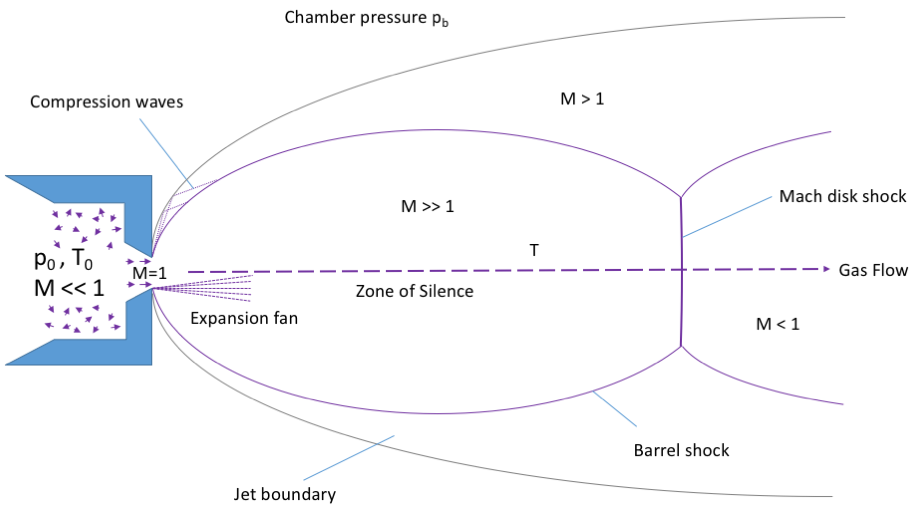
\includegraphics[width=1.00\textwidth]{images/freeJetExpansion.png}
	\caption[Schematic of a supersonic gas expansion into a vacuum.]{Schematic of a supersonic gas expansion into the vacuum. Gas is stored in a reservoir at pressure $p_{0}$, temperature $t_{0}$ and speed of the gas is thermal distributed $\left(M\ll 1\right)$. As the gas enters the nozzle area, it is accelerated to the speed of sound $\left(M=1\right)$ and as the gas expands, the temperature T drops altering the speed of sound such that the gas now travels supersonic $\left(M\gg 1\right)$. In this expansion, clusters are generated in the nozzle region, where $M=1$ (see text for details). After \citep{Miller-1988-Oxford}}
	\label{fig:freeJetExpansion}
\end{figure}
Supersonic jet setups typically store gas in a reservoir at a certain stagnation pressure $p_{0}$ and temperature $T_{0}$. The gas expands through a nozzle into a vacuum and figure \ref{fig:freeJetExpansion} shows a schematic drawing of this process. Typical values for $p_{0}$ are 10 bars, where the mean free path of the atoms is much smaller than the nozzle diameter D. This is why many collisions occur during the expansion in the nozzle and the above described kinetic theory explains the cluster formation. However, this holds not true in the supersonic molecular flow region, where no further cluster growth happens. To understand the expansion process in detail, we assume to work with an ideal gas and to describe the gas expansion itself, we further assume that no clusters are formed and that turbulence and effects of heat conduction are unimportant \cite{Yamada-2001-SciDir,Haberland-1994-Springer}.\\
To begin, the velocity distribution of the gas is thermally distributed at a set temperature $T_{0}$. The movement direction of each atom is randomly orientated. For an ideal gas, we can define the enthalpy $H_{0}$ in the stagnation chamber
\begin{align}
H_{0}=c_{p} T_{0},
\intertext{with the specific heat $c_{p}$ for atoms}
c_{p}=\frac{5}{2}k_{B},
\label{eq:stagnation-enthalpy}
\end{align}
where is the Boltzman constant $k_{B}$. The expansion of the gas through the nozzle is driven by the pressure difference $p_{vac}/p_{0}$. In the nozzle, the (steady) gas flow becomes directed and the enthalpy $H_{0}$ is converted into kinetic energy $\frac{1}{2}m v^{2}$ and a rest enthalpy $H$. So, in the expansion process, we can use the conservation of energy, and equation \eqref{eq:stagnation-enthalpy} we can write down
\begin{equation}
H_{0}=H+\frac{1}{2}m_{gas} v^{2} = c_{p}T+\frac{1}{2}m_{gas}v^{2},
\label{eq:local-temperature}
\end{equation}
with $T$ being the local temperature along the gas flow and $m_{gas}$ the atomic mass of the gas. To look at this in greater detail, let us define the Mach number $M$ as the ratio of the stream velocity $v$ and the local speed of sound $c_{s}$
\begin{equation}
c_{s}=\sqrt{\frac{\gamma k_{B} T}{m_{gas}}}.
\label{eq:local-speed-of-sound}
\end{equation}
With the ratio of specific heats $\gamma = \frac{c_{p}}{c_{v}}$ at constant pressure and volume, they can be regarded as independent of temperature for atomic gases, we can rearrange equation \ref{eq:local-temperature} to 
\begin{equation}
T=T_{0}\left(1+\frac{1}{2}\left(\gamma - 1\right)M^{2}\right)^{-1}.
\label{eq:local-temperature-definition}
\end{equation}
Here the interplay between the Mach number $M^{2}$ and the local temperature $T$ give insight into the directed mass flow versus the remaining thermal energy in the system. As indicated the the figure \ref{fig:freeJetExpansion}, M increases dramatically along the expansion axis and that is due to decrease in speed of sound $c_{s}$ that is proportional to $\sqrt{T}$ as indicated in equation \eqref{eq:local-speed-of-sound}\footnote{In other words, the gas is expanding and quickly reaches the terminal velocity $v_{\infty}=\sqrt{\frac{2 R}{m_{gas}}\left(\frac{\gamma}{\gamma-1}\right) T_{0}}$, with $R$ being the universal gas constant, while the speed of sound is decreasing. This can be abused to calculate flight times $t_{\text{flight}}=\frac{d}{v_{\infty}}$, if the distance $d$ from nozzle to interaction point is known.}. Finally, this attribute has given the name to supersonic jets.\\
Let us describe the appearance of the jet stream (see figure \ref{fig:freeJetExpansion}) next. Upon exiting the nozzle, the Mach number increases by a wide margin ($M\gg 1$), that means that the gas travels faster than information in this medium. Here, a \textit{zone of silence} is formed, where the gas flow is not influenced by other particles, thus uninterrupted. As the supersonic flow is exiting the nozzle it has to turn around the edge of the nozzle to further expand and the supersonic flow turns by actually creating smaller Mach waves. At the borders of the \textit{zone of silence}, $M$ decreases drastically resulting in dense regions that are called \textit{barrel shock} to the sides and \textit{Mach disk} downstream the gas flow. For an unhindered transport of the gas and clusters to the interaction region, the interaction region needs to be within the \textit{zone of silence}. We can express the distance from the nozzle to the Mach disk $x_{MD}$ through
\begin{equation}
\frac{x_{MD}}{d}=0.67\sqrt{\frac{p_{0}}{p_{b}}},
\label{eq:distance-of-mach-disk}
\end{equation}
with the nozzle diameter $d$. So the competing stagnation pressure $p_{0}$ and the background pressure $p_{b}$ define the distance of the otherwise static parameters. $p_{b}$ needs to be low enough do drive the Mach disk downstream of the interaction region. By using skimmers and thereby physically separating the jet expansion into separately pumped compartments, the background pressure $p_{b}$ can be reduced, hence $x_{MD}$ increased.\\
While we have described a cooling gas in the expansion process it should be noted that the clusters are comparably hot. Through the kinetic process described above, they are efficiently heated. The two processes to loose energy are, one, collisions with a chaperone $M$ that deactivates the cluster, or two, evaporation of monomers from the cluster. The evaporation process makes the temperature size-independent, after the clusters have reached a certain minimum size \cite{Farges-1981-SurfSci}. Typically, the jet reaches temperatures of a few Kelvin and the cluster temperature is heavily dependent on their material, particularly the dissociation energy. For this study relevant are mostly the temperature of Xenon cluster that is $~75K$\footnote{To put this temperature in perspective, krypton clusters are $~50K$ and argon cluster $~40K$ \cite{Farges-1981-SurfSci,Gspann-1986-Springer}. Note that in this study the cluster size was $\bar{N} > 800$, hence above the minimum value to be size independent. For the evaporative cooling process to settle at a given temperature, a certain flight distance (in the cited study 6.5cm) should also be taken into account.} and the fact xenon clusters are solid as their melting temperature is higher \cite{Gspann-1986-Springer}. For similar reasons, helium clusters are liquid, which is why they are often called (helium-)droplets. If helium droplets are produced using a cryogenic jet even superfluid helium-droplets can be observed.\\
\begin{table}
	\centering
		\begin{tabular}{ | l | l | l | l | l | }
			\hline
			Helium & Neon & Argon & Krypton & Xenon \\ \hline
			3.85 & 185 & 1646 & 2980 & 5554 \\ \hline
		\end{tabular}
	\caption[Parameter $K_{\text{gas}}$ values for rare gases.]{Parameter $K_{\text{gas}}$ values for rare gases \cite{Schorb-2012-Thesis}.}
	\label{tab:k-parameter}
\end{table}
At the current point of the discussion, it should shine out that the average cluster size\index{cluster size} is very much depended on the gas type, stagnation temperature $T_{0}$, stagnation pressure $p_{0}$ and the nozzle type. Indeed, an empirically found scaling law\index{scaling law} named after Hagena\index{Hagena|see {scaling law}} \cite{Hagena-1972-JCP,Hagena-1981-SurfSci,Hagena-1987-ZeitschriftAMC}, can be written down as
\begin{equation}
\Gamma^{*} = K_{\text{gas}} \cdot T_{0}^{0.25q-1.5} \cdot p_{0} \cdot d_{eq}^{q},
\label{eq:Hagena-parameter}
\end{equation}
with the gas specific parameter $K_{\text{gas}}$ that can be found in table \ref{tab:k-parameter} for some rare gases, the gas specific parameter $q$ that varies between 0.5 and 1 and is 0.85 for all rare-gases, and the equivalent nozzle opening $d_{eq}$ that is $d_{eq}=d$ for pinhole sources and for conical nozzles $d_{eq}$ reads
\begin{equation}
d_{eq} = d\frac{\tan\left(\Phi_{0}\right)}{\tan\left(\Phi\right)}
\label{eq:equivalent-nozzle-opening}
\end{equation}
with the half opening angle of the nozzle $\Phi$ and the half opening of the free gas expansion $\Phi_{0}$. The Hagena scaling parameter $\Gamma^{*}$\index{Hagena!scaling parameter} allows us to estimate the mean cluster size, i.e. amount of accumulated particles per cluster $<N>$, as follows
\begin{itemize}
	\item $\Gamma^{*} < 350$, no cluster formation observed.
	\item $350 < \Gamma^{*} < 1800$, in this region $<N>$ reads
		\begin{equation}
		<N> = 38.4 \left(\frac{\Gamma^{*}}{1000}\right)^{1.64}
		\label{eq:intermediate-hagena-scaling}
		\end{equation}
	\item $1800 < \Gamma^{*}$, in this region $<N>$ reads
		\begin{equation}
		<N> = 33.0 \left(\frac{\Gamma^{*}}{1000}\right)^{2.35}
		\label{eq:large-hagena-scaling}
		\end{equation}
\end{itemize}
Supersonic jets generally create clusters of different sizes. This size distribution is centered around $<N>$ and for solid rare gas clusters this distribution is a log-normal distribution. The size distribution can be an experimental challenge, especially when size dependent effects are investigated. Historically, electron diffraction \cite{Farges-1981-SurfSci,Bartell-1986-ChemRev} has been used to determine the mean cluster size, mean temperature and mean geometry. Today, free electron laser allow the determination of the size of a single cluster through a diffraction image and by measuring enough single clusters, one can reproduce size distributions of a supersonic jet as shown in figure \ref{fig:size-distributions}.\\
Experiments using supersonic jets for cluster generation are typically performed with pulsed valves to decrease cost and gas load in the overall system. Upon opening and closing of the valve, the gas density varies. This mostly affects the cluster size and one would expect to see smaller clusters. This remains true in the beginning of the pulse but in the \textit{afterpulse}\index{afterpulse} one finds giant clusters that exceed the above described scaling laws due to the effects when closing the valve \cite{Rupp-2014-JCP}.
%
%
%
%
%
\subsection{Creation of a heterogeneous cluster}
%%%%%%%%%%%%%%%%%
%- Heterogeneous clusters, e.g. He Xe\\
%- Do you have literature on that?
%%%%%%%%%%%%%%%%%
\begin{figure}
	\centering
		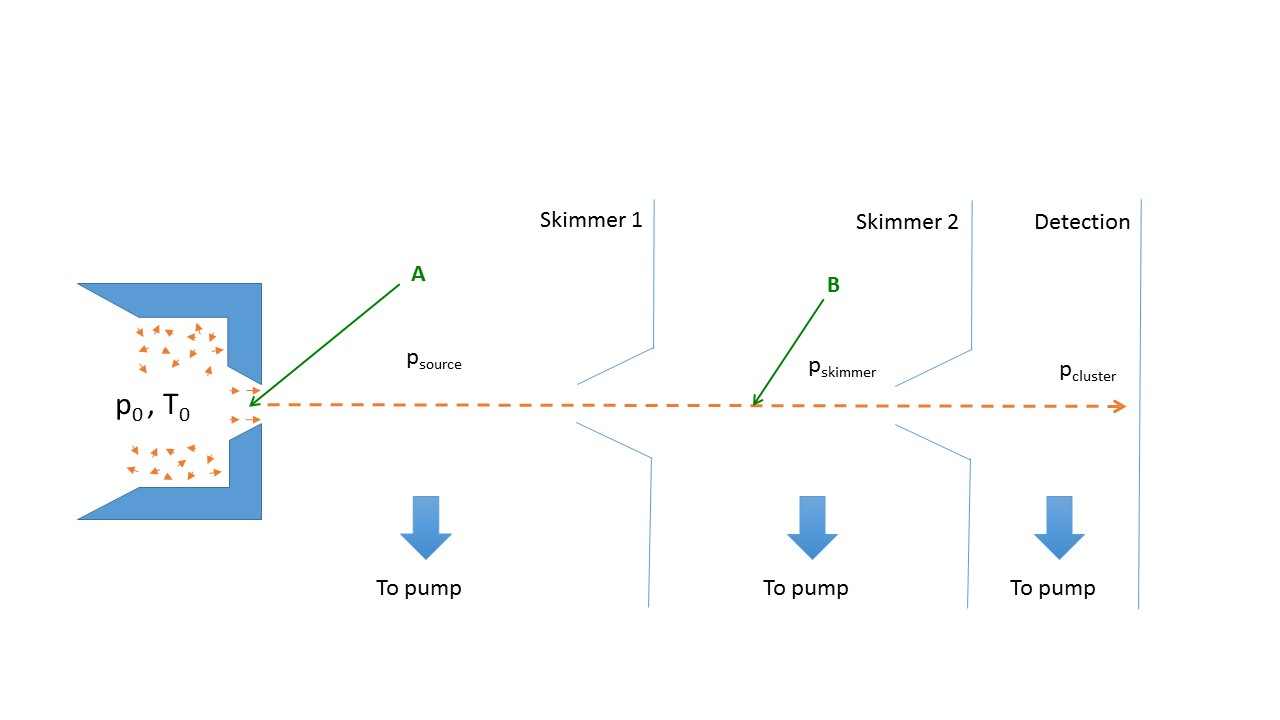
\includegraphics[width=1.00\textwidth]{images/pick-up.jpg}
	\caption[Schematic of a pickup (gas-)source.]{Schematic setup to generate heterogeneous clusters through pickup. Thereby is a first cluster generated via a supersonic gas expansion, which is doped at regions marked A or B. In region A, the dopant gas is mixed in the nozzle such that it becomes part of the nucleus. In region B, the cluster condenses atoms on its surface and commonly gas cells are used to regulate the pressure $p_{\text{skimmer}}$ effectively. $p_{\text{source}}$ is the pressure in the source chamber. The cluster can be detected upon evaporation, i.e. by contact with the chamber, through the pressure $p_{\text{cluster}}$ and the cluster doping can be determined through partial pressures (see text for details). After \cite{Gough-1985-JChemPhys,Haberland-1994-Springer}.}
	\label{fig:pickupPrinciple}
\end{figure}
A possibilities to create heterogeneous clusters is through the principle of picking-up atoms or molecules \cite{Gough-1985-JChemPhys,Haberland-1994-Springer}. Figure \ref{fig:pickupPrinciple} illustrates pickup regions that are typically used in an experiment. Mainly, there are two different pickup places, one, monomers are added to the cluster in region A of figure \ref{fig:pickupPrinciple} that represents the nozzle of a supersonic source, or two, they can be picked up by a cluster in region B for example through an increased background pressure $p_{b2}$ with the dopant material. If clusters pick up atoms or molecules in the nozzle region A, they can become part of the cluster formation and can be found inside of solid clusters. If atoms or molecules are picked up in region B, they stick to the surface of solid clusters. If a (super-)liquid cluster picks up a dopant, it may move within the droplet. Since the traversing cluster is much larger and heavier than a colliding monomer the trajectory is not affected significantly. Already pressures of $p_{b2}=10^{-11}$ bars over a pickup length of a few centimeters can dope the cluster in significant form. At these low pressures, picking up atoms or molecules in region B requires less gas load on the system but is also less efficient than picking up in region B. To increase the pickup levels in region B, a gas cell can be used as much higher pressures can be achieved within the gas cell without putting too much gas-load on the overall system.\\
The collision with the cluster and a dopant\index{dopant} does add energy to the cluster just as the cluster growth process itself. This is why the initial cluster will loose particles through evaporation upon pick up of a dopant \citep{Gomez-2011-JCP}. The loss of particles through evaporative cooling is dependent on the ratio of dissociation energies of the two materials and can be written down as
\begin{equation}
N_{\text{Evaporated from cluster}} \approx \frac{\epsilon_{\text{cluster}}}{\epsilon_{\text{dopant}}},
\label{eq:evaporated-amount}
\end{equation}
with the dissociation energy of the cluster $\epsilon_{\text{cluster}}$ and of the dopant $\epsilon_{\text{dopant}}$. In the case, where a helium droplet is doped with xenon atoms, we may use the dissociation energies of helium $\epsilon_{He}=0.6\cdot 10^{-3}$ eV and xenon $\epsilon_{Xe}=0.6\cdot 10^{-3}$ eV \citep{Gomez-2011-JCP,Gomez-2014-Science}, such that approximately 250 helium atoms evaporate by picking up 1 xenon atom.\\
We can extend this idea to estimate the amount of picked-up atoms, if we were to know the amount of atoms in the cluster before and after the pickup area. An estimate of the initial cluster size $\left\langle N_{\text{cluster}}\right\rangle$ can be reached through the scaling laws\footnote{As already established the actual cluster size produced with a supersonic jet will vary, hence the average cluster size $\left\langle N_{\text{cluster}}\right\rangle$.} as discussed in section \ref{sec:homogenous-cluster}. A measure to estimate the cluster size after the pickup can be established through measuring the partial pressure of the cluster material $p_{\text{cluster}}$ of helium\footnote{For example with a residual gas analyzer.}, when the particle jet hits a wall and evaporates (see figure \ref{fig:pickupPrinciple}). The partial pressure $p_{\text{cluster}}$ then scales linearly with the initial cluster size $\left\langle N_{\text{cluster}}\right\rangle$, such that
\begin{equation}
\left\langle N_{\text{dopant}}\right\rangle \approx \frac{\epsilon_{\text{cluster}}}{\epsilon_{\text{dopant}}} \cdot \frac{\Delta p_{\text{cluster}} \left\langle N_{\text{cluster}}\right\rangle}{p_{\text{cluster}}},
\label{eq:average-dopant}
\end{equation}
where $\Delta p_{\text{cluster}}$ denotes the partial pressure difference with pickup and without.
%%%
%\section{Introduction into X-ray scattering}\label{sec:scattering-theory}
%%%%%%%%%%%%%%%%%%%%%
%- Starting with Maxwell equations (this would be coming from the far end, I might be able to go into Guiniers formalism earlier. Depending on space.)\\
%- Mathematical model for electromagnetic wave\\
%- Kramers-Kronig relations\\
%- Mie scattering in a nutshell
%%%%%%%%%%%%%%%%%%%%%%%
%
\section{Light-matter interaction}\label{sec:light-matter-interaction}
A full description of light-matter interaction is mathematically challenging and not the purpose of this thesis. In the following subsections, we will break down the light-matter interaction into its components. The components of the interaction of photons with matter can be split into fife categories, 1) coherent-elastic scattering (see sub-section \ref{sec:saxs}), 2) inelastic processes (absorption, see sub-section \ref{sec:absorption}), 3) incoherent scattering (Compton effect) and high-energy physics effects of 4) pair production and 5) absorption effects with the nucleus. As it already shines through, the effects are dependent on the wavelength and the cross-sections for 3-5 can be neglected in the soft X-ray regime. We will therefore concentrate the discussion on points 1-2 and restrict ourselves to the for the experiment necessary theory.
%This section will give  a brief introduction into the elastic scattering of X-rays with matter. The actual scattering process is very complex as it is an interplay of coherent, incoherent and elastic, inelastic processes. Fortunately, we can reduce the scattering description to its main process: The coherent and elastic scattering. In other words, we neglect Compton scattering (incoherent), any kind of absorption processes (inelastic) and effects form the scattering of multiple particles. We will then start this section by looking at the small angle scattering of atoms and continue on to extended objects such as clusters. The section is rounded off by an introduction to the inverse problem and basic algorithm ideas to overcome the issue of phase retrieval.
%Photons can also be absorbed by atoms in which case an electron get either excited to another state or ionized. At X-ray wavelengths matter typically gets ionized in the inner shells. Upon absorption a cascade of relaxation processes begins and the now ionized atom finds the new most energetic favorable state. These processes are particularly depended on the wavelength of the incident photons but also the type of atom. This chapter is devoted to these processes and particular the absorption process is described in section \ref{sec:absorption} and the relaxation processes in \ref{sec:relaxation}.
%
%
%
\subsection{Small angle X-ray scattering}\label{sec:saxs}
%%%%%%%%%%
%- Switch to Guiniers approximation and description\\
%- Work towards small angle scattering of small particles\\
%- Particular spheres\\
%- Discuss extreme positions
%%%%%%%%%%%
We can describe a linear polarized, electric field of a continuous electromagnetic wave via the following expression \citep{Als-Nielson-2011-JWS}
\begin{equation}
\vec{E}(\vec{r},t) = \vec{\epsilon} E_{0} e^{i \vec{k}\cdot\vec{r}},
\end{equation}
with $\vec{E}(\vec{r},t)$ being the electromagnetic field of the wave, the wave vector $\vec{k}$, the Cartesian coordinate vector $\vec{r}$, the complex amplitude if the electric field is then $E_{0}\exp^{i \vec{k}\cdot\vec{r}}$ and because of the polarization we use $\vec{\epsilon}$ such that $\vec{\epsilon}\cdot\vec{k}=\vec{k}\cdot\vec{E}=\vec{k}\cdot\vec{H}=0$. Through a relative comparison, of the incoming intensity $I_{0}$ and the scattered intensity $I_{\text{sc}}$, we can phenomenological establish the differential cross-section over a certain solid angle $\Delta \Omega$ as
\begin{align}
\left(\frac{d\sigma}{d\Omega}\right)&=\frac{\left(\text{Number of X-rays scattered per second into $\Delta \Omega$}\right)}{\left(\text{Incident flux}\right)\left(\Delta\Omega\right)}=\frac{I_{sc}}{\left(I_{0}/A_{0}\right)\Delta\Omega},
\label{eq:scattering-crosssection}
\end{align}
with $A_{0}$ being the covered area of the incident beam. If an electro-magnetic wave encounters an electron, we can describe the scattering semi-classical by imagining how an electron starts to oscillate once it sees an incoming electric wave. The electron then functions as a dipole antenna eventually radiating the wave into a certain solid angle $\Delta \Omega$. Depending on the polarization of the incident beam we can reduce equation \ref{eq:scattering-crosssection} to \citep{Als-Nielson-2011-JWS}
\begin{align}
\left(\frac{d\sigma}{d\Omega}\right)&=r_{0}^{2}P,
\intertext{with the classical electron radius $r_{0}=2.82\ 10^{-5}\text{\AA}$ and the polarization factor P}
P&=\begin{cases}
1& \text{vertical scattering plane},\\
\cos^{2}\left(\Psi\right)&\text{horizontal scattering plane},\\
\frac{1}{2}\left(1+\cos^{2}\left(\Psi\right)\right)& \text{unpolarized source.}
\end{cases}
\end{align}
We can now move on and use this knowledge for atoms, where we have Z electrons. To describe electrons in an atom, let us proceed by introducing the electron density $\rho_{e}\left(\vec{r}\right)$ that describes the probability density of electrons in an atom. Figure \ref{fig:X-ray-scattering} illustrates the scattering process in one atom. An incident beam with wave number $\vec{k}$ is elasticly scattered at a point $\vec{r}$ into a wave with $\vec{k}'$ such that $\left|\vec{k}\right|=\left|\vec{k}'\right|$. In this wave picture, the scattering process must be seen as a superposition of waves and it is particular illustrated how the wave scattered at the origin of the atom is scattered as well. As both waves are scattered at different points, they have an optical path difference $2 \delta$. This difference in path length results in a phase difference to each other and eventually leads to interference between the waves. So, we can describe the phase difference $\Delta \Phi\left(\vec{r}\right)$ of the waves scattered at $\vec{r}$ and the origin by
\begin{equation}
\Delta \Phi\left(\vec{r}\right) = \left(\vec{k}-\vec{k}'\right)\cdot \vec{r} = \vec{Q} \cdot r,
\label{eq:phase-difference}
\end{equation}
with $\vec{Q}$ being denoted as the \textit{wave vector transfer}\index{wave vector!transfer}. Through trigonometry, we can establish the more common denotation of the wave-vector $\vec{Q}$
\begin{equation}
\vec{Q}=2 \left|\vec{k}\right| \sin\left(\frac{\Theta}{2}\right)=\frac{4 \pi}{\lambda}\sin\left(\frac{\Theta}{2}\right),
\label{eq:Q-scattering-angle}
\end{equation}
with the wavelength of the light $\lambda$ and the scattering angle $\Theta$.\\
A volume element $d\vec{r}$ at $\vec{r}$ will now scatter depending on its electron density, namely by $-r_{0}\rho\left(\vec{r}\right)d\vec{r}$. At scattering angle $\Theta=0$, i.e. $\vec{Q}=0$ the atomic form factor $f^{0}$ is
\begin{equation}
f^{0}\left(\vec{Q}\rightarrow 0\right)=Z,
\label{eq:transform-number-of-particles}
\end{equation}
because all scatterer are in phase. As we increase the scattering angle $\Theta$, the phase difference $\Delta \Phi\left(\vec{r}\right)$ leads to interference, which we can describe by multiplying a phase factor $e^{i \vec{Q}\cdot \vec{r}}$ to the electron density $-r_{0}\rho\left(\vec{r}\right)d\vec{r}$. In the limit of $\vec{Q}\rightarrow\infty$, the atomic form factor then is $f^{0}\left(\vec{Q}\rightarrow\infty\right)=0$. We can integrate over the total scattering length, and write down
\begin{equation}
-r_{0} f^{0}\left(\vec{Q}\right)=-r_{0}\int\rho_{e}\left(\vec{r}\right)e^{i \vec{Q}\cdot \vec{r}}d\vec{r}.
\label{eq:scattering-integral}
\end{equation}
\begin{figure}
	\centering
		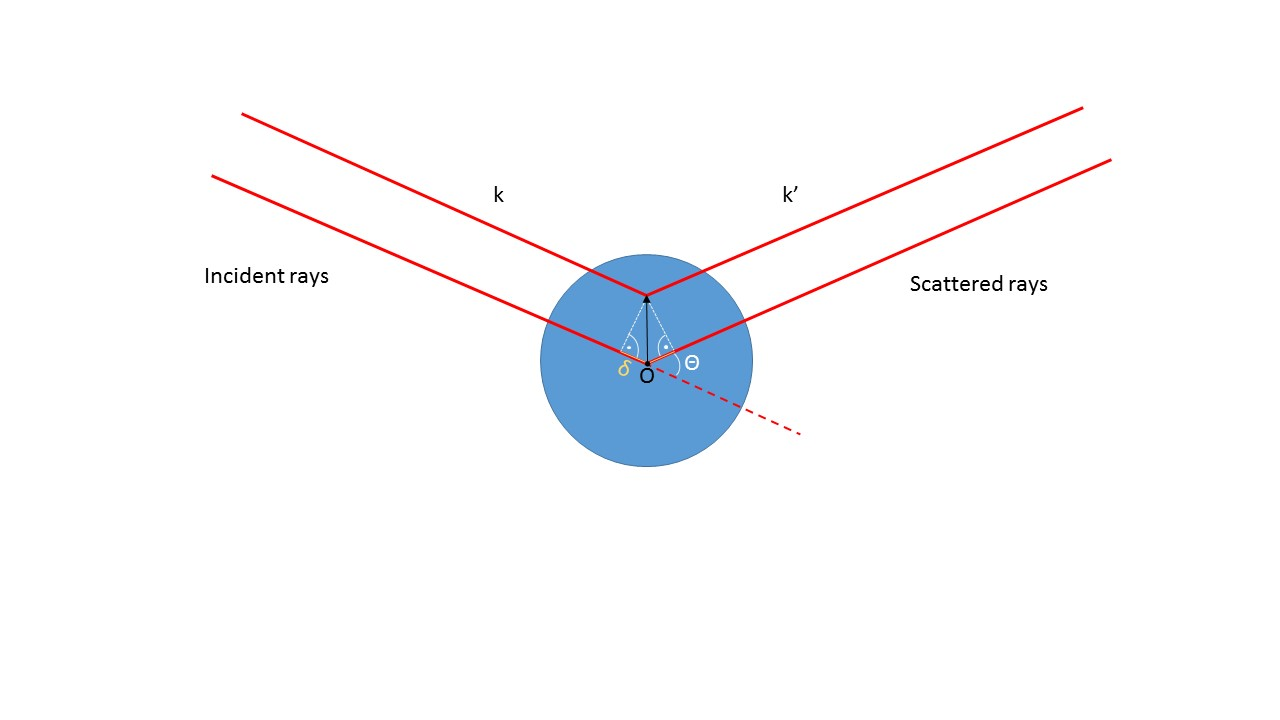
\includegraphics[width=1.00\textwidth]{images/X-ray-scattering.jpg}
	\caption[Principle of scattering rays of an atom.]{Principle of scattering rays of an atom. After \cite{Als-Nielson-2011-JWS,Guinier-1955-JWS}.}
	\label{fig:X-ray-scattering}
\end{figure}
This important result is called the atomic form factor and it can be understood as a Fourier transform of the electron density of an atom. We can also remember from optics the light scatter of an object can be inverse Fourier transformed and projects an image of the object again.\\
Let us continue with the scattering of a molecule or cluster that consist of multiple atoms. We can label the atoms in such an object by
\begin{equation}
F^{object}\left(\vec{Q}\right)=\sum_{j}f_{j}^{0}\left(\vec{Q}\right)e^{i \vec{Q}\cdot \vec{r}},
\label{eq:scattering-factor-object}
\end{equation}
with the atomic form factors $f_{j}^{0}\left(\vec{Q}\right)$ for the $j$'th atom and call $-r_{0} F^{object}$ the scattering length of the object. Strictly speaking and as defined, $F^{object}\left(\vec{Q}\right)$ is $\vec{Q}$ depended. As this is inconvenient, let us consider the following evidence in order to neglect this dependency. In the angular range of $\vec{Q}$, where $F^{Object}\left(\vec{Q}\right)$ is not 0, $f_{j}^{Q}\left(0\right)$ can be considered constant \citep[see][p. 6-7]{Guinier-1955-JWS}. In human hemoglobin, the range in which the molecule (object) scattering length is not 0, the carbon atomic form factors change less than $0.4$\%. It is therefore most convenient to describe the scattering length of extended objects via one continuous electron density, where certain volume elements $d\vec{r}$ scatter proportional to their electron density $\rho_{e}\left(\vec{r}\right)$. We can therefore go forward with a continuous description of extended objects using a generalized electron density $\rho\left(\vec{r}\right)$. Let us gather the last results in the following expression for the scattering length of an object
\begin{equation}
-r_{0}F^{O}=-r_{0}\int \rho\left(\vec{r}\right) e^{i \vec{Q}\cdot r}d\vec{r},
\label{eq:scattering-factor-general}
\end{equation}
and we can see that it is mostly the phase factor that yields information about the structure of the object as it is the phase factor that constitutes the diffraction pattern.\\
The total scattered intensity $I\left(\vec{Q}\right)$ in a diffraction pattern can expressed through
\begin{equation}
I\left(\vec{Q}\right)=\left|A\right|^{2}=I_{0}\left|F^{0}\left(\vec{Q}\right)\right|^{2},
\label{eq:scattered-intensity}
\end{equation}
where an incident beam with intensity $I_{0}$ with a complex amplitude $A$\index{amplitude!complex} performs an operation that can be interpreted as a Fourier transform of the objects electron density. The process of measuring the scattered light, for example through a detector, merely measures the modulo of an amplitude $\left|A\right|^{2}$, which eliminates the phase factor $e^{i\Delta\Phi\left(\vec{r}\right)}\cdot e^{-i\Delta\Phi\left(\vec{r}\right)}=1$. In order to reconstruct the object that scattered in realspace, e.g. to understand its shape or to study its function, we need to recover the for the structure most important phase information. We will discuss iterative algorithms that can recover phase information in section \ref{sec:phase-retrieval}.\\
Let us briefly address the scattering of a rare-gas cluster, as the cluster can be considered as a spherical symmetric object. That allows to express the electron density of a cluster with radius $R$ as 
\begin{align}
\rho\left(\vec{r}\right)&=\begin{cases}
1& \text{for $R \geq \vec{r} \geq 0$},\\
0&\text{for $R > \vec{r}$}.
\end{cases}
\label{eq:el-density}
\end{align}
Using equation \eqref{eq:el-density}, we can solve the integral in equation \eqref{eq:scattering-factor-general} by transforming into spherical coordinates
\begin{align}
F_{\text{Sphere}}^{O}\left(\vec{Q}\right) &= \int_{0}^{\pi}\int_{0}^{2\pi}\int_{0}^{R} r^{2}  sin\left(\Theta\right) e^{i \vec{Q} r \cos\left(\Theta\right)} dr d\Theta d\Phi\\
&=\frac{\sin\left(\vec{Q} R\right)-\vec{Q} R\cos\left(\vec{Q} R\right)}{\vec{Q}^{3} R^{3}}=\frac{J_{1}\left(\vec{Q}R\right)}{\vec{Q}R},
\label{eq:scattering from sphere}
\end{align}
with $J_{1}$ being the Bessel function of first kind. Formula \eqref{eq:scattering from sphere} can be easily abused to determine the size of a spherical particle using local minima in the diffraction pattern\footnote{Equation \eqref{eq:scattering from sphere} can be solved numerically for the distance between the first two minima, where $\Delta\vec{Q}R=3.24$, such that $R=\frac{3.24}{\vec{Q}_{\text{min}^{n+1}}-\vec{Q}_{\text{min}^{n}}}$} or through a numerical fit of the resulting curve.
%
%
%\subsection{X-ray diffraction}
%- I wonder if I should include this to talk about 'what happens on faster timescales' using Ken's work.
%
%
%
%
\subsection{Ionization of matter}\label{sec:absorption}
Let us quickly remember the atomic scattering factor $f^{0}\left(\vec{Q}\right)$, which we were able to introduce by neglecting a variety of (wavelength depended) effects through Fourier transforming the electron density of an atom. If we imagine (soft) X-rays approaching an atom classically, we can compare it to the analogon to a forced harmonic oscillator, where an electric field drives a (bound) electron. As a result, the phase velocity of light $v_{\text{phase}}$ is reduced to the speed of light in vacuum $c$ through interacting with electrons. Hence we would think of an increase in the refractive index $n=c/v_{phase}$\index{refractive index}. Also, if the the energy of the photons is higher than binding energies of electrons in the atom then also a probability for dissipation/absorption exists \citep{Als-Nielson-2011-JWS,Attwood-2007-CUP}. These two effects are connected to the atomic scattering factors $f^{0}\left(\vec{Q}\right)$ and are called dispersion corrections to the atomic scattering factor. Let us include these corrections as a atomic form factor
\begin{equation}
f\left(\vec{Q},\hbar\omega\right)=f^{0}\left(Q\right)+f'\left(\hbar\omega\right)+i f''\left(\hbar\omega\right),
\label{eq:scattering-factor-dispersion-corr}
\end{equation}
where $f'\left(\hbar\omega\right)$ corrects for the phase velocity and the wave amplitude correction/absorption $f''\left(\hbar\omega\right)$. In the limit of high photon energies $\hbar \omega$ the electrons can be largely seen as free, as the binding energies become a little factor, and $f'\left(\hbar\omega\right)\rightarrow 0$ and $f''\left(\hbar\omega\right)\rightarrow 0$. As the photon energies $\hbar \omega$ are closer to the atomic level, which is the case at soft X-rays for many materials, $f'\left(\hbar\omega\right)$ and $f''\left(\hbar\omega\right)$ can become large factors. Note particularly that these corrections only apply to the forward scattering, where $\vec{Q}=\Theta=0$.\\
We shall not derive this relation in its full extend that can be read in \citep[see][p. 55ff]{Attwood-2007-CUP}, but we shall compare the equation for the complex refractive index $n\left(\omega\right)$ to these arguments. Let us start by imagining a electromagnetic wave propagating in a medium. The wave propagating in a medium along the axis $z$ can be written as
\begin{equation}
e^{i n k z}= \underbrace{e^{i \left(1-\delta\right)k z}}_{\text{phase shift}}\underbrace{e^{-\beta z}}_{absorption},
\label{eq:wave-in-medium}
\end{equation}
\begin{figure}
	\centering
		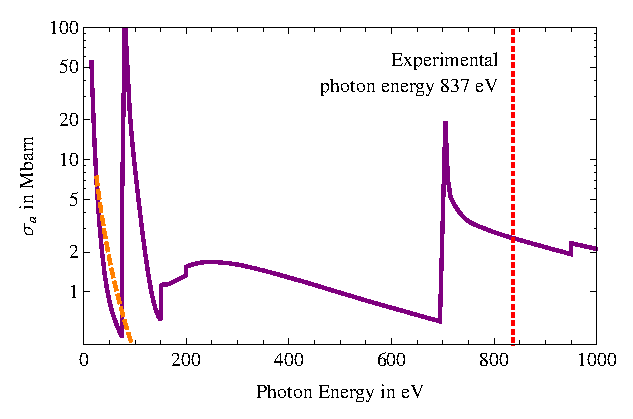
\includegraphics[width=1.00\textwidth]{images/photoionization.eps}
	\caption[Total absorption cross-sections for helium and xenon.]{Total absorption crosssections $\sigma_{a}$ in megabarn for xenon and helium. The purple curve represents the total cross-section of xenon. The orange dashed curve represents the total cross-section of helium. The red dashed line represents the photon energy used at the experiment described in the present work. Data points from \citep{Elettra-2016-Website,Yeh-1985-AtmDat,Yeh-1993-GBSP}}
	\label{fig:photoionization}
\end{figure}
where $n$ is the complex refractive index, $\delta$ the real dispersion correction\index{dispersion correction!complex} resulting in a phase shift of the wave and $\beta$ being the imaginary dispersion correction resulting in a decline in amplitude of the wave\footnote{We jump between wave and particle picture as it pleases us. Here, a decline in amplitude in the wave picture can be read as absorption in the particle picture.}. The relation between the complex refractive index, $\beta$ and $\delta$ is explicitly given by
\begin{equation}
n\equiv \frac{c}{v_{\text{phase}}}=1-\delta+i\beta.
\label{eq:complex-refractive-index}
\end{equation}
Let us now jump to the result of the forced harmonic oscillator calculation given in \citep[p.~278]{Als-Nielson-2011-JWS} and realize that we are allowed to define this dispersion relation through the atomic form factor as \citep[see][p.~76]{Als-Nielson-2011-JWS}
\begin{equation}
n\equiv 1- \frac{2\pi \rho_{atom}r_{0}}{k^{2}}\left(f^{0}\left(\vec{Q}=0\right)+f'\left(\hbar\omega\right)+f''\left(\hbar\omega\right)\right),
\label{eq:eq:complex-refractive-index-atomic-factors}
\end{equation}
with the atomic number density $\rho_{atom}$ and we identify
\begin{align}
\delta &= \frac{2 \pi \rho_{atom} r_{0}}{k^{2}}\left(f^{0}\left(\vec{Q}=0\right)+f'\left(\hbar\omega\right)\right),\quad \text{and}\\
\beta &= - \left(\frac{2\pi \rho_{atom}r_{0}}{k^{2}}\right)f''\left(\hbar\omega\right).
\label{eq:delta-and-beta}
\end{align}
We have already established that $\beta$ reduces the amplitude of the incoming wave through absorption. Thus, using the insight gained from the absorption part in equation \eqref{eq:wave-in-medium}, we can rewrite equation \eqref{eq:delta-and-beta} and define $f''\left(\hbar\omega\right)$ in terms of being proportional to an absorption cross section $\sigma_{a}$, which reads
\begin{equation}
f''\left(\hbar\omega\right)=-\left(\frac{k}{4\pi r_{0}}\right)\sigma_{a}.
\label{eq:f-2-definition}
\end{equation}
Figure \ref{fig:photoionization} shows the total absorption cross-sections $\sigma_{a}$ for xenon, helium under which a bound electron absorbs a photon and excited into the continuum, thus the atom is ionized\index{photoionization}. To get a better understanding of the fundamental absorption related details about xenon and helium, table \ref{tab:xenon-photoionization-cross-section} and \ref{tab:helium-xenon-ionization} show the differential photo-absorption cross sections and ionization potentials for various energy levels and each ionization configurations, respectively, at the photon energy $837$ eV. The calculations were performed using the Los Alamos Atomic Physics code based on \citep{Cowan-1981-Cal}.
\begin{table}
	\centering
		\begin{tabular}{ | c | c | c | c | }
			\hline
			Shell & Subshell & Cross-section & subshell ionization \\
				&	& in Mb & potential in eV \\ \hline
			K & 1s & - & 34630.0 \\ \hline
			L & 2s & - & 5466.4  \\ 
			\ & 2p & - & 4899.1 \\ \hline
			M & 3s & - & 1153.3  \\ 
			\ & 3p & - & 965.4 \\ 
			\ & 3d & 2.2505 & 682.7 \\ \hline
			N & 4s & 0.0305 & 223.7 \\ 
			\ & 4p & 0.1247 & 161.8 \\ 
			\ & 4d & 0.2587 & 68.2  \\ \hline
			O & 5s & 0.0040 & 27.3  \\ 
			\ & 5p & 0.0120 & 12.5  \\ \hline
		\end{tabular}
	\caption[Differential absorption cross-sections and ionization potentials for xenon.]{Differential absorption cross-sections and ionization potentials for certain electronic configurations of xenon at 837eV. Calculations based on \citep{Cowan-1981-Cal}.}
	\label{tab:xenon-photoionization-cross-section}
\end{table}
It appears that certain energy levels, or here subshells if one disregards the hyperfine structure\footnote{A shift in energy levels due to interaction of electrons with the nucleus \citep[see][p~166~ff.]{Demtroder-2005-Springer}.}, tend to have a higher absorption cross-section than others. This brings us back to the picture of the forced harmonic oscillator, where an electron is driven by a light field. If the frequency of the light field is close to the eigenfrequency of the bound electron, in other words, if the energy of a photon is close to the energy level of a bound electron, the system is in resonance and absorption is highly likely. As the photon energy and electron level energy differ, the system is off resonance and it is less likely to absorb a photon. As energy levels in atoms are discrete, electrons can only be excited from one energy level to another or need a certain (minimal) ionization energy\index{ionization!energy} to ionize an atom and excite an electron into the continuum. The likelihood of a core-electron that is strongly bound being ionized is by far the most probable using X-rays.
\begin{table}
	\centering
		\begin{tabular}{ | c | c | c | c | }
		\hline
%			Configuration & ionized subshell & Cross-section (Mbarn) & Helium ionization potential in eV \\ \hline
			El. Configuration, & Ionization & Cross-section  & subshell ionization  \\
			and ionized subshell & of subshell & $\sigma_{a}$ in Mbarn & potential in eV \\ \hline
			He\textsuperscript{+0},\ 1s2 & 1s2 & 0.0007 & 24.4 \\ \hline
			He\textsuperscript{+1},\ 1s1 & 1s1 & 0.0005 & 54.4 \\ \hline
			Xe\textsuperscript{+0},\ 5p6 & 3d10 & 2.2505 & 682.7 \\ \hline
			Xe\textsuperscript{+1},\ 3d9 & 3d9 & 2.1487 & 733.6 \\ \hline
			Xe\textsuperscript{+1},\ 5p5 & 3d10 & 2.2443 & 693.7 \\ \hline
			Xe\textsuperscript{+2},\ 5p4 & 3d10 & 2.2390 & 705.9 \\ \hline
		\end{tabular}
	\caption[Absorption cross-sections and ionization potentials for xenon and helium]{Absorption cross-sections $\sigma_{a}$ and ionization potentials for certain electronic configurations, including certain ionization profiles. Calculations based on \citep{Cowan-1981-Cal}.}
	\label{tab:helium-xenon-ionization}
\end{table}
When a core electron gets ionized, the electronic structure changes and particular ionization energies and (absorption) cross-sections change. To discuss the parameters that are most applicable to this thesis, a comparison of the most probable transition at the photon energy 837eV is given for helium and xenon in table \ref{tab:helium-xenon-ionization}. The ionization energies change drastically, whether one ionizes are core electron or a less tight bound electron. Similarly to the back-on-the envelope calculation given in equation \eqref{eq:absorption-cross-section}, it is very unlikely to an atom to absorb more than two photons in one pulse of a free electron laser, which is why we only consider the most probably transitions here to get an understanding how the absorption cross-sections change.\\
% \begin{table}
% 	\centering
% 		\begin{tabular}{ | c | c | c | c | }
% 		\hline
% 			El. Configuration, & Ionization & Cross-section  & subshell ionization  \\
% 			and ionized subshell & of subshell & $\sigma_{a}$ in Mbarn & potential in eV \\ \hline
% 			Xe\textsuperscript{+0},\ 5p6 & 3d10 & 2.2505 & 682.7 \\ \hline
% 			Xe\textsuperscript{+1},\ 3d9 & 3d9 & 2.1487 & 733.6 \\ \hline
% 			Xe\textsuperscript{+1},\ 5p5 & 3d10 & 2.2443 & 693.7 \\ \hline
% 			Xe\textsuperscript{+2},\ 5p4 & 3d10 & 2.2390 & 705.9 \\ \hline
% 		\end{tabular}
% 	\caption{caption. Calculations based on \citep{Cowan-1981-Cal}.}
% 	\label{tab:xenon-ionization}
% \end{table}{}
The total elastic scattering cross-sections for neutral and ionized helium and xenon can be found in table \ref{tab:helium-xenon-el-scattering-crossection}. It is interesting to see that although xenon has only 27 times more electrons than a helium atom the scattering factor $f^{0}$ of neutral xenon is over 900 times stronger helium. Upon ionization, the absolute changes in $f^{0}$ of helium are therefore smaller compared to xenon. However, the relative change in helium of $f^{0}$ by getting one of two electrons ionized ~75\% and ionized helium barely scatters. As xenon has multiple occupied subshells, the scattering factors of different ionized subshells are shown. As discussed, it is most likely to ionize the 3d subshell but subsequent relaxation processes\footnote{See the following section \ref{sec:relaxation}.} lead to a ionized 5p subshell. For the scattering factor, there is little change whether the 3d or 5p subshell becomes ionized and the change in $f^{0}$ is only ~0.05\%. As xenon has 54 electrons, the relative change upon ionization of one electron in $f^{0}$ is only 3\% and small compared to helium, which allows us to conclude that xenon scatters still well after ionization.  
\begin{table}
	\centering
		\begin{tabular}{ | c | c | }
		\hline
			El. Configuration, & Scattering factor \\
			and ionized subshell & $f^{0}$ in barn \\ \hline
			He\textsuperscript{+0},\ 1s2 & 2.5539  \\ \hline
			He\textsuperscript{+1},\ 1s1 & 0.649465  \\ \hline
			Xe\textsuperscript{+0},\ 5p6 & 1874.36  \\ \hline
			Xe\textsuperscript{+1},\ 3d9 & 1813.56  \\ \hline
			Xe\textsuperscript{+1},\ 5p5 & 1814.68  \\ \hline
			Xe\textsuperscript{+2},\ 5p4 & 1754.08  \\ \hline
		\end{tabular}
	\caption[Atomic scattering factors for helium and xenon.]{Atomic scattering factor $f^{0}$ for certain electron configurations. Calculations based on equation \eqref{eq:scattering-integral}. From \cite{Ho-2016-PC}}
	\label{tab:helium-xenon-el-scattering-crossection}
\end{table}
In the experiment described in the following chapters, the photon energy is explicitly chosen to have a comparably high absorption cross-section for xenon but is off absorption resonance, a comparably low absorption cross-section for helium and a wavelength short enough to receive high resolution images through coherent diffraction imaging. In such a setting xenon is most likely to absorb X-rays rather than helium. Thus given the raw absorption likelihoods, the xenon atoms (and clusters) are most prone to X-ray induced dynamics. Let us now have a look at these dynamics in atoms and study the electronic relaxation processes in atoms upon absorption of an (X-ray) photon.
%
%
%
%
%
\subsection{Charge migration}\label{sec:relaxation}
%%%
\begin{figure}
	\centering
		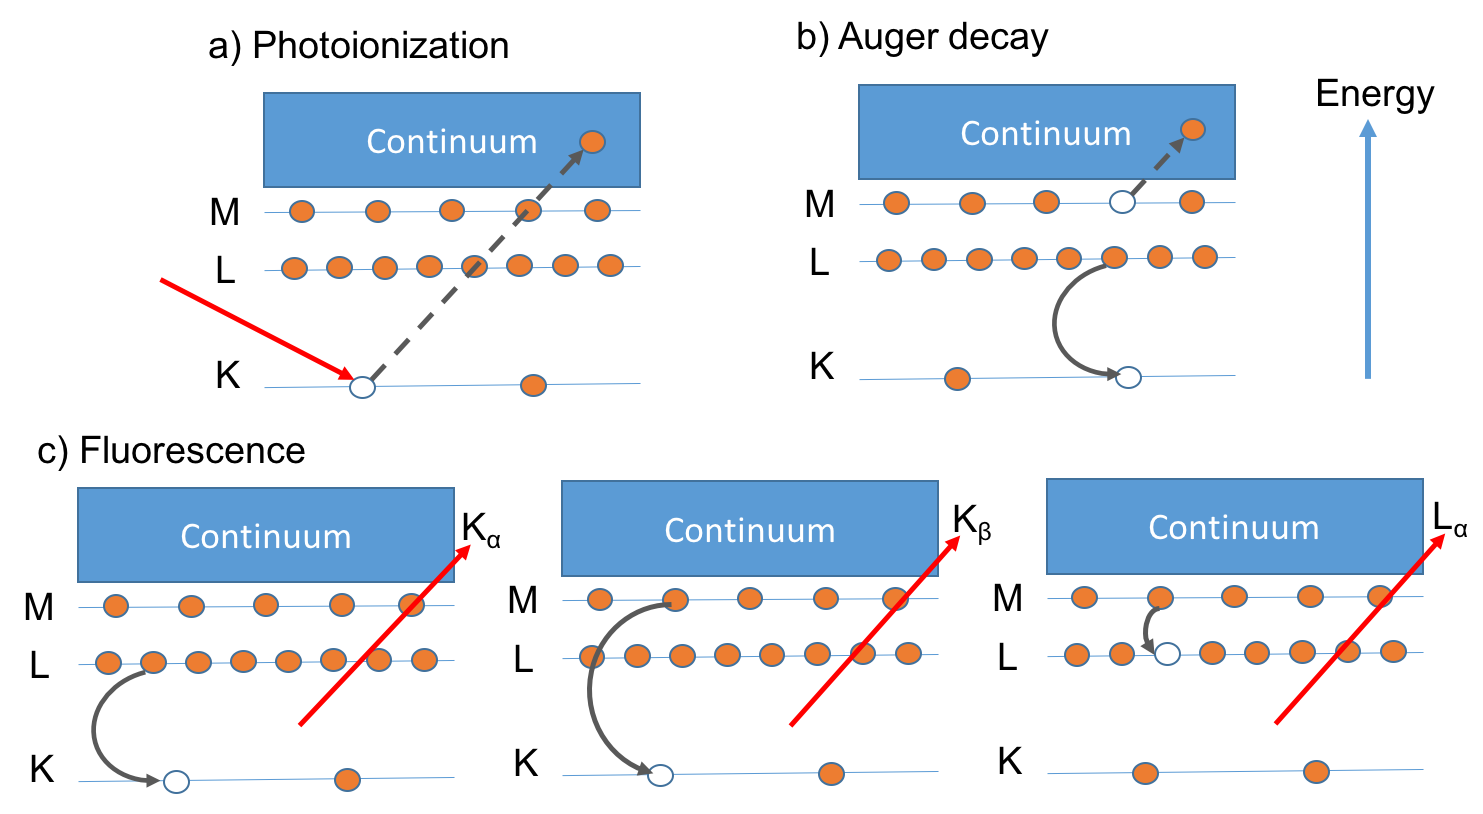
\includegraphics[width=1.00\textwidth]{images/el-relaxation.png}
	\caption[Schematic illustration of common charge transfer processes]{Schematic illustration of common charge transfer processes. a) describes a direct emission of an K-shell electron after absorbing a X-ray photon. Process b) shows a secondary relaxation process called Auger decay, where a K-shell hole is filled with an electron from the L-shell and the remaining energy is released through emission of an electron in an outer shell, here M-shell, into the continuum. Process c) illustrates fluorescence, where an electron hole is filled with an electron from an outer shell and the remaining energy is released through photons. Process a) has a destinct spectra depending on the ionized element and the wavelength of the absorbed photon, the released particles in b-c) show an element specific spectra. After \citep[][p.~19]{Als-Nielson-2011-JWS}}
	\label{fig:el-relaxation}
\end{figure}
After an atom has been (core-)ionized due to absorption of a photon as depicted in figure \ref{fig:el-relaxation}a, the atom is not in its most energetically favorable state. In order to emit energy and transition into its new ground state, the atom can emit particles according to the schematics in figure \ref{fig:el-relaxation}b-c. The electron hole in the (K-)shell created due to absorption of a photon above ionization threshold is filled by an electron in a energetically higher shell, here L or M shell, and thereby emits a photon of the discrete energy of the difference between the transitioning levels. The discrete lines are thus element specific and modern photoemission spectroscopy can yield insight into for example element identification, excitation dynamics or chemical bonds.
\begin{figure}
	\centering
		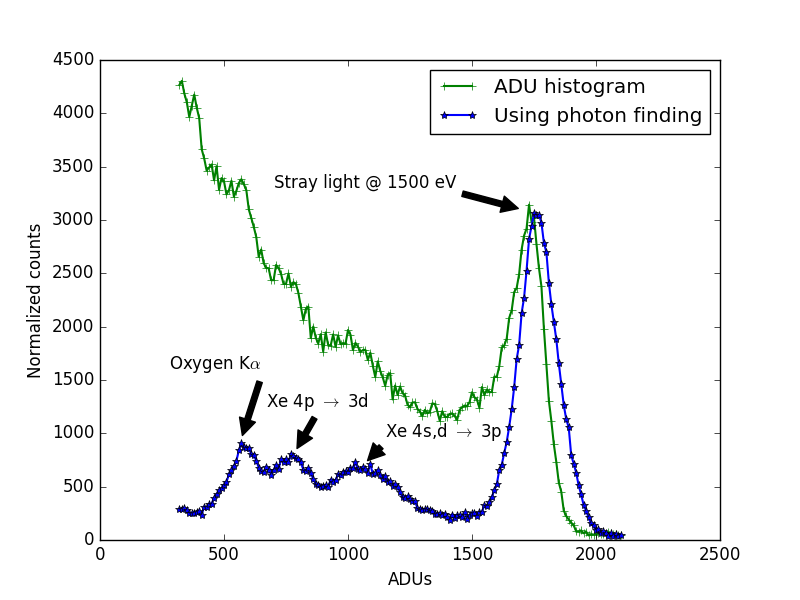
\includegraphics[width=.49\textwidth]{images/pnCCD-histogram.png}
		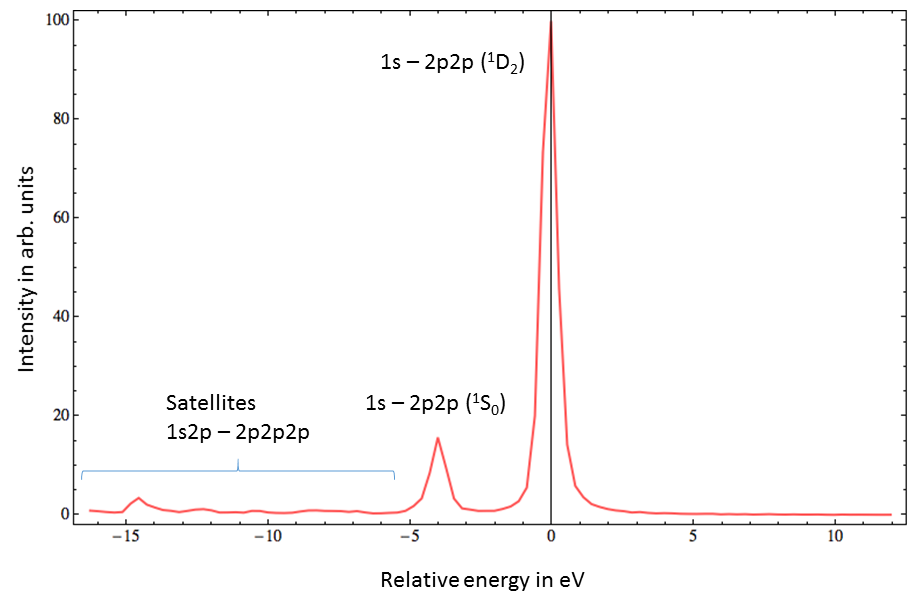
\includegraphics[width=.49\textwidth]{images/auger-spectra.png}
	\caption[Fluoresence spectra from xenon and neon K-LL Auger spectrum.]{Left spectra shows fluorescence peaks from xenon and oxygen illuminated with 1.5keV photons from the LCLS and detected with pnCCD detectors \citep{Bucher-2016-Unpublished, Rudek-2012-NatPho}. The green curve is a ADU histogram of the pnCCD detector and the blue curve uses a coalescent photon finder as described in section \ref{sec:pnccd-corr}. Right, selection of the K-LL Auger spectrum with rel. energy 0 corresponding to 804.5eV. The ionization starts in the K shell, i.e. a 1s hole, and the Auger relaxation process ends up with two holes, e.g. in the L-shell denoted as LL or 2p2p. As electrons energy levels arrange due to their quantum numbers, multiple peaks appear for similar hole configurations, e.g. 2p2p \cite{Bucher-2014-Unpublished,Krause-1970-PhysLettA}.}
	\label{fig:pnCCD-histogram}
\end{figure}
Figure \ref{fig:pnCCD-histogram} left shows measured fluorescence lines of oxygen and xenon. In this measurement, xenon atoms and residual oxygen atoms have been illuminated with 1500 eV photons from the Linac Coherent Light Source and the fluorescence photons has been measured with the LAMP pnCCD detectors described in section \ref{sec:pnCCD}. The green curve is a ADU histogram of the pixel-detector using the detector calibrations described in section \ref{sec:pnccd-corr}. The blue curve additionally uses a photon-finding algorithm as the signal from just one fluorescence photon splits up into multiple pixel. An algorithm then looks for pixel above a certain threshold and includes neighboring pixel above a certain threshold, thus correcting the measured signal to yield a proper fluorescence yield.\\
Another possibility for the atom to emit absorbed energy is through a 2-step process, where an outer shell electron is emitted into the continuum, the so called Auger-electron\footnote{Named after the french physicist Pierre Auger.} and simultaneously another electron fills the electron-hole. Emitted Auger-electrons have discrete energies depending on the combination of electrons involved in the process and can therefore help identifing elements or be used to calibrate energies. Figure \ref{fig:pnCCD-histogram} right shows a partial K-LL Auger spectrum from neon illuminated by soft X-ray pulses from LCLS and measured with a hemispherical analyzer as described in \citep{Bucher-2014-Unpublished}. Neon is ionized in the K-shell and electron-hole in 1s is created. In the Auger decay, an electron from the L-shell fill the 1s hole and another electron from the L-shell is emitted into the continuum. As there is a variety of electronic configurations that can be involved in this process multiple peaks appear for similar configurations, e.g. 1s - 2p2p. More complex structures, called satellites, appear when the initial ionization configuration is more complex, e.g. KL-LLL satellites. An Auger decay occurs typically on the few femtosecond timescale \citep{Krause-1970-PhysLettA}.\\
Similar to the Auger decay, where electrons from an outer shell are involved in the relaxation process, the transition can also be of the same shell and is then called a Coster-Kronig transition. Relevant transitions are for example the N-NN Coster-Kronig transitions in xenon \citep{Coster-1935-Physica}.
\\
So far we have looked at X-ray induced processes from atoms. Extended objects, whether a bio-molecule or a cluster, will respond differently than just the atoms they consist of. Nanometer-sized objects will develop a distinct character due to their electronic bond with other particles. This includes rare-gas clusters that are weakly bound Van der Waals forces. We shall explore this behavior in the next section \ref{sec:ionizatin-of-ext-obj}.
%
%
%
%
\section{Ionization of clusters in intense X-ray pulses}\label{sec:ionizatin-of-ext-obj}
%%%%%%%%%%%%%%%%%%%
%- Short introduction coming from inelastic scattering
%%%%%%%%%%%%%%%%%%%
The response of a cluster in intense X-rays differs from just the atomic response. Collective effects change the microscopic (sample) environment and it is now the collective of atoms that generates a response to the strong FEL pulse.
\subsection{Formation and expansion of a nanoplasma}\label{sec:nanoplasma-expansion}
%%%%%%%%%%%%%%%%%%%%%%%%
%- Step by step explanation on the formation of a nanoplasma
%%%%%%%%%%%%%%%%%%%%%%%%
\begin{figure}
	\centering
		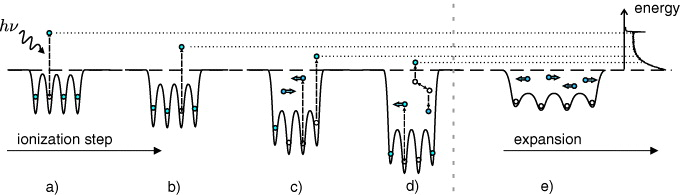
\includegraphics[width=1.00\textwidth]{images/nano-plasma-schematic.jpg}
	\caption[Schematic of the nanoplasma creation and expansion.]{Schematic of the nanoplasma creation and expansion. In step a) X-ray photons ionize electrons from a cluster. b) subsequent \textit{multistep ionization}\index{ionization!multistep} try to relax the electronically excited system, deepening the Coulomb potential of the cluster. Step c) shows a deepened Coulomb potential of the cluster, due to which the multistep ionization becomes (partially) frustrated and electrons are trapped in the potential. In step d) trapped electrons collide and start to thermalize. Collisions can lead to emission of trapped electrons. d) The superheated nanoplasma starts to expand. From \citep[\href{https://creativecommons.org/licenses/by/3.0/}{\ccby}]{Arbeiter-2011-NJP}}
	\label{fig:nano-plasma-schematic}
\end{figure}
 Let us begin by recapture the elastic, coherent scattering part of the response that has been discussed in sub-section \ref{sec:saxs}. Equation \eqref{eq:scattering-factor-object} indicates how the scattering length of a cluster can be calculated and, neglecting inelastic processes, this remains elastic scattering response holds true. If we consider the inelastic effects discussed in section \ref{sec:absorption}, it should be clear that the elastic scattering length -$r_{0}F^{Object}$ is reduced due to the (atomic) dispersion corrections $f'\left(\omega\right)$ and $f''\left(\omega\right)$ that reduce the scattering length $-r_{0}f^{0}\left(\vec{Q}\right)$ of a single atom. The dominating change in scattering length is driven by the photo ionization process introduced via $f''\left(\omega\right)$. We follow the figure \ref{fig:nano-plasma-schematic} and \citep{Arbeiter-2011-NJP,Bostedt-2010-JPB} in the next five steps. Step a) of the nanoplasma transition\index{nanoplasma!transition}, the cluster gets ionized due to intense radiation\footnote{The wavelength of radiation must be above the ionization threshold of at least one subshell, however, it must not be X-rays with a wavelength on the nanometer length scale.}. Step b), further ionization through emission of photo electrons and Auger electrons lead to a so called \textit{multistep ionization}\index{ionization!multistep} that steepens the Coulomb potential\index{Coulomb potential} \citep{Wabnitz-2002-Nature,Laarmann-2004-PRL,Bostedt-2008-PRL}. Step c), the multistep ionization is suppressed (or frustrated) because the Coulomb potential depth is larger than the atomic excess energy of photo- and Auger electrons. The emitted electrons are now trapped in the cluster potential and are \textit{quasi-free}. Upon increasing \textit{inner ionization}\index{ionization!inner} the nanometer sized object undergoes a phase transition to a nanoplasma\footnote{Plasma is another state of matter, similar to solid, liquid and gaseous, where molecular bonds dissociate and positive and negative particles are present in increasing numbers.}. Step d), the temperature of the nanoplasma is initially defined by the atomic excess energies (a rather discrete spectrum) but collisions with other particles lead a (kinetic) energy distribution of the electrons that is similar to thermal distributions and can be measured via the spectra of evaporated electrons \citep{Laarmann-2005-PRL,Bostedt-2010-NJP}. Step e) Hydrodynamic and Coulomb forces drive an expansion of the cluster and the cluster will ultimately disintegrate. The hydrodynamic portion of the force is due to the increasing hot plasma and the resulting increase outward pressure, whereas the the Coulomb portion comes from the repelling force of same charges. Both these forces reasonably describe the expansion process, are not exclusive and depend mostly on sample size and irradiation technique.\\
Regarding the sample size, large clusters efficiently trap electrons in their Coulomb potentials such that the quasi-free electrons thermalize and subsequently heat the nucleus. The hot nanoplasma system then tries to expand due to the increase in internal pressure. Electrons thermalize on the attosecond timescale and simulations show that the energy transfer to the ions can be as fast as 50 fs \citep{Arbeiter-2010-PRA}. Small clusters trap photo and Auger electrons less efficiently and electrons are free such that the heating process is suppressed. In this case, the ions see the repelling force due to Coulomb interaction of same charges with each other \citep{Lezius-1998-PRL}.\\
Following a similar line of argumentation, low energy ionizing photons allow efficient trapping of photo and Auger electrons, thus favorable conditions for a hydrodynamic expansion. Conversely, high photon energies\footnote{Meaning hard X-ray with wavelenghs on the {\AA}ngstrom length scale as soft X-rays have similar photon energies as trapping potentials and multistep ionization deepens the Coulomb potential enough.} lead to more atomic excess energy such that more electrons overcome the trapping potential, thus favorable conditions for a Coulomb expansion. However, this line is very element depended and atoms with large atomic mass, such as Xenon\footnote{Find ionization energies for specific subshells in table \ref{tab:xenon-photoionization-cross-section} and deepened Coulomb potential ionization energies after ionization of Xe, here Xe$^+1$ and Xe$^{+2}$ for different subshell ionization configurations, in table \ref{tab:helium-xenon-ionization}.} would require photon energies $E_{ph}$ of $5.5keV\ll E_{ph} < 34.6k eV$ or $34.6keV\gg E_{ph}$ and since mostly the immediate process upon photon absorption is wavelength depended and the electron trapping of the majority of subsequent multistep ionizations will be mostly depended on the cluster size. It remains to discuss the radiation intensity and the more intense the ionizing radiation is, the more electrons are ionized per time-step such that the intensity of the light mainly drives the time needed for a cluster to undergo the phase-transition to a nanoplasma, expand and disintegrate.\\
\subsection{Imaging of transient states}
\begin{figure}
	\centering
		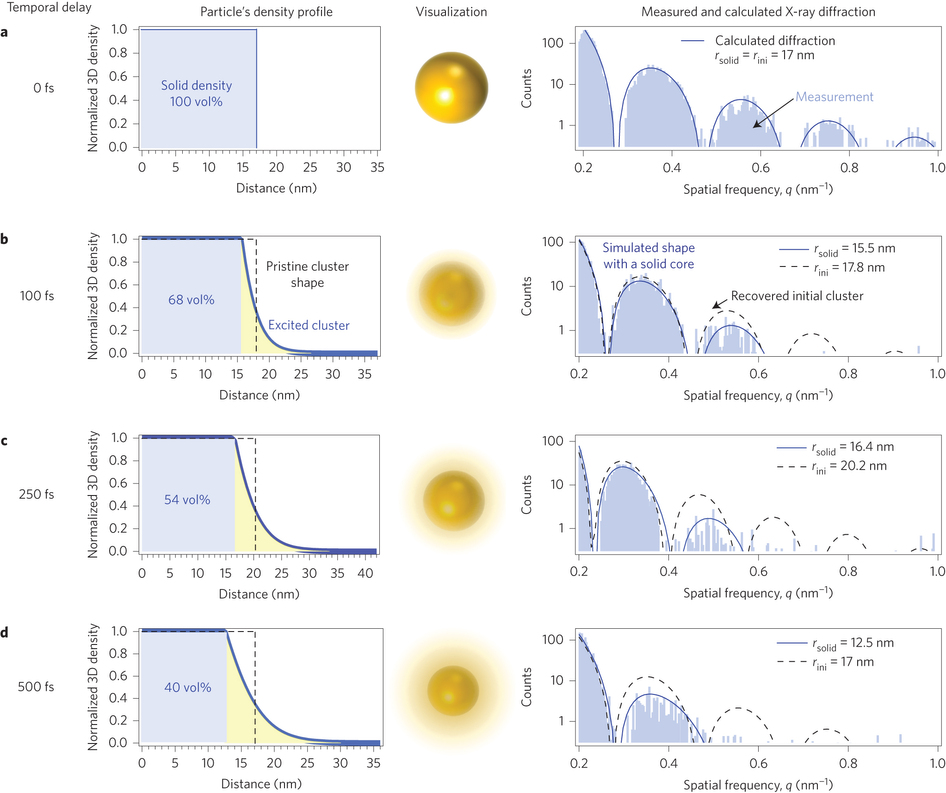
\includegraphics[width=1.00\textwidth]{images/tais-nat-photonics.jpg}
	\caption[Measurement and simulation of the nanoplasma expansion in xenon cluster.]{Left series, simulation of of diffraction patterns. Right series, measured diffraction patterns of (spherical) xenon clusters pumped with an NIR laser pulse and probed a certain time delay with an LCLS pulse. The diffraction pattern show a decrease in intensity at larger q values, which can be explained through an expanding electron densities, i.e. a nanoplasma expansion. Electron density simulations are performed in 1D and the densities Fourier transform is fitted to the measurement for a solid sphere (dashed line) and an expanding sphere (solid line). From \citep{Gorkhover-2016-NatPho}. Reprinted with permission from Nature Publishing Group.}
	\label{fig:tais-nat-photonics}
\end{figure}
The reason why the nanoplasma transition is important is because every matter irradiated by a free-electron laser will undergo the nanoplasma transition and finally disintegrate. This is particular challenge for structural biology \citep{Neutze-2000-Nature} as sample damage due to the FEL x-ray pulse changes the desired structure one ought to investigate. In order to prevent falsified measurements, one needs to understand the nanoplasma transition as it occurs while the pulse is propagating through the sample. First attempts to perform a combined spectroscopic and imaging technique revealed correlations between the complex refractive index\index{refractive index!complex} \citep{Bostedt-2012-PRL} and the diffraction patterns but also correlations of the ion spectroscopic data and the diffraction patterns intensity \citep{Gorkhover-2012-PRL}. More recently, simulations on diffraction patterns could show the expanding electron density \citep{Gorkhover-2016-NatPho} as it is also shown in figure \ref{fig:tais-nat-photonics}. In this particular study, an infra-red laser was used start (pump) a nanoplasma transition in a xenon cluster and subsequently image (probe) this state with a XFEL pulse. As the time delay between pump and probe pulse is varied, the resulting diffraction patterns of the 15-20 nm Xe-cluster show declining intensities at larger scattering angles with increasing time delay $\Delta t>100 fs$. The loss in signal could be explained through an expanding electron density\index{electron density!expanding} \citep{Hau-Riege-2008-PRE,Peltz-2014-PRL}. The electron density thereby expands increasingly over time due to the Coulomb and Hydrodynamic forces and, first the outer layers expand and at larger time delay also the inner atomic layers. In this study, an electron temperature of 200eV could be measured in this study by comparing plasma simulations to the ion spectroscopy signal. The possible spatial resolution out of the diffraction patterns has been estimated to be 8 nm but through assuming a shape the electron density model is sensitive below this resolution.\\
\begin{figure}
	\centering
		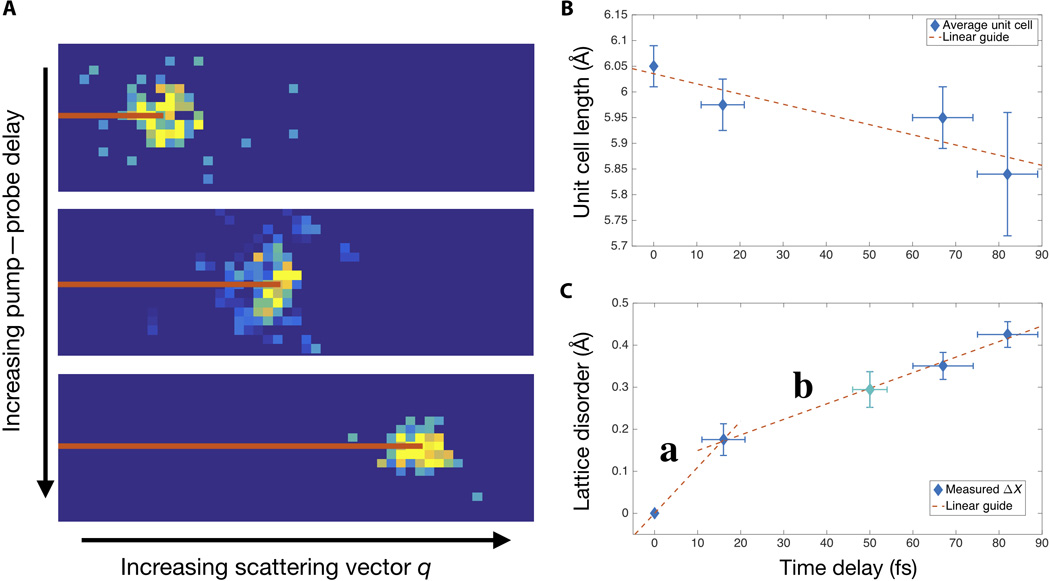
\includegraphics[width=1.00\textwidth]{images/ken-science.jpg}
	\caption[Experiment that shows early evolution of the nanoplasma transition.]{X-ray pump -- X-ray probe scattering experiment on Xe-cluster that shows an early evolution of the nanoplasma transition. A, single-shot Bragg peaks at varying time delays. The scattering vector q increases over time delay. B, unit cell length over time delay. The unit cell length decreases, therefore the cluster shrinks in size. C, Lattice disorder over time delay. The measured fcc lattice is becoming disordered after being pumped with a X-ray pulse. From \citep{Ferguson-2016-SciAdv}. Reprinted with permission from AAAS.}
	\label{fig:ken-science}
\end{figure}
At shorter time delays $\Delta t<100 fs$ xenon cluster compress in size \citep{Ferguson-2016-SciAdv}. Since clusters form as a crystal\footnote{See section \ref{sec:homogenous-cluster}.}, one can determine their structure through crystallographic approaches as it is explained in full detail in \citep[][chapter 5]{Als-Nielson-2011-JWS}\footnote{In short, crystals scatter light and through interference when fulfilling the, so called, Bragg-law $m \lambda = 2d \sin\left(\Theta\right)$, with $m$ being an integer, $\lambda$ being the wavelength of the scattered light, $d$ the distance between crystalline layers and $\Theta$ the scattering angle. When Bragg's condition is fulfilled, the rays interfere constructively and signal can be detected. Similar to small angle scattering, the image of the crystal is best expressed in reciprocal space where $d$ can be connected to $a$ and $\Theta$ to $q$ (or $\vec{Q}$ as denoted earlier) such that a structure can be determined.}. Figure \ref{fig:ken-science}a is showing how the signal from fulfilling Bragg's law\index{Bragg's law} over the scattering vector $q$. The signal moves to larger scattering vectors $q$ and, as $q=\frac{2\pi}{a}$, the unit cell length $a$ is shrinking over the time delay $\Delta t = \{0,..,100\}$. This unintuitive and contradictory result is attributed to the changes in electronic configuration upon ionization. Electrons that are trapped in the cluster Coulomb potential have an increased mobility and are able to contribute comparable to valence electrons to the chemical bonding. As a result, the unit cell, i.e. the crystalline structure, changes on the {\AA}ngstrom length scale and the lattice becomes increasingly disordered (see figure \ref{fig:ken-science}c). Conversely, this stand in stark contrast with the experiment explained above. The nanoplasma transition is therefore a multistep process in which first the initial ionization occurs, followed by an increased Coulomb potential that traps electrons, which then change the structure of the nanosample. Eventually, the system becomes strongly ionized and hot such that Coulomb and hydrodynamic forces disintegrate the cluster into it's atomic components.
%
%
%
\subsection{Tampered layers to inhibit the nanoplasma expansion}
%%%%%%%%%%%%%%
%- Step by step explanation on the formation of the nanoplasma, pointing out the differences between tampered and pristine clusters
%
%
%%%%%%%%%%%%
Initially, it was proposed that very short pulses outrun radiation damage\index{radiation damage} processes \citep{Neutze-2000-Nature}. Pulses from the XFEL must be shorter than the lifetime of Auger processes, thus on few femtosecond long, to outrun the multistep ionization\index{ionization!multistep}. It shall also be noted here that limiting the XFEL pulse duration, e.g. at LCLS\index{LCLS}, limits the pulse energy\index{pulse energy} and therefore the overall scattered intensity. However, outrunning radiation damage does not circumvate photoionization and it is therefore said that short pulses only reach a certain resolution \citep{Aquila-2015-StrucDyn}. So, it is a particular question, whether electron densities and here particular bonding configuration are obtainable by solely outrunning radiation damage. As radiation damage is unavoidable it can be mitigated in several ways. As the underlying processes are well understood, one way to mitigate for the radiation damage would be to computer model the effects, however, this can only be done for small particles. Another way to fundamentally increase resolution in single particle imaging is due to prior alignment of particles such that their orientation is know. While this has seen some success for small molecules \citep{Kupper-2014-PRL}, it is currently unknown, whether this works for larger molecules as the strong light fields, which are needed to align the molecules, may change their structure. Recent advances with phase-reconstruction algorithms made it possible to computationally determine the orientation of the particle at the time of imaging \citep{Loh-2009-PRE,Ekeberg-2015-PRL} without prior knowledge if at least a few hundred images are provided. Thus, making molecule alignment a niche application. In this thesis, we shall discuss a method to reduce effects of damage is through artificial tampered layers. Artificial shells around a sample supply it with electrons and function as sacrificial layer that protects the sample \citep{Hau-Riege-2010-PRL}. For aerosol particles, this method has also only been investigated through ion spectroscopy \citep{Hoener-2008-JPB,Ziemkewitz-2017-unpublished}.
\begin{figure}
	\centering
		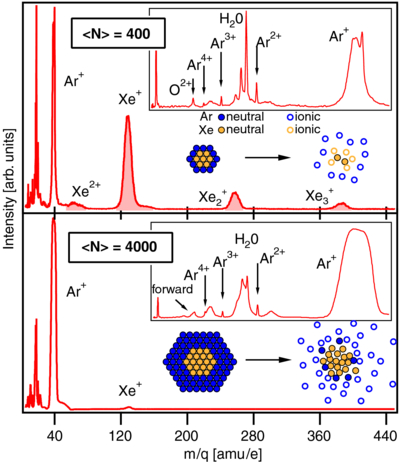
\includegraphics[width=0.50\textwidth]{images/Hoener-image.jpg}
	\caption[Time of flight spectra of argon and xenon core-shell systems.]{Time of flight (TOF) traces of argon and xenon core shell systems irradiated with 93eV X-ray pulses from FLASH\index{Free electron LASer in Hamburg!FLASH}. At this energy, mostly Xe is ionized and the ionized atoms create strong Coulomb potential that traps electrons towards the center of the cluster. The top panel shows smaller clusters with 400 particles, in which the trapping is inefficient, few electron-ion recombinations occur, thus Xe and Ar ions are detected in the TOF detector. The bottom panel shows large clusters with 4000 particles and thicker argon shell, here Xe-ions recombine in the center and the TOF shows mostly Ar ions as the neutral Xe remains undetected. at different sizes. From \citep[\href{https://creativecommons.org/licenses/by/3.0/}{\ccby}]{Hoener-2008-JPB}.}
	\label{fig:Hoener-image}
\end{figure}
In the study shown in figure \ref{fig:Hoener-image} a core-shell system of argon and xenon was constructed and, here, the xenon compares to the sample and the argon compares to the sacrificial layer around the particle (see figure). The heterogeneous cluster were irradiated with 93eV photons from \textit{FLASH}\footnote{Short for \textbf{F}ree electron \textbf{LAS}er in \textbf{H}amburg. An extreme ultra violet (XUV) free electron laser in Hamburg, Germany.}\index{Free electron LASer in Hamburg!FLASH} at which mostly xenon atoms are ionized. As described in the nanoplasma creation process (see section \ref{sec:nanoplasma-expansion}), the increasing ionized cluster creates a steep Coulomb potential trapping electrons. Trapped electrons are available for recombination with the ionized atoms. In the small core-shell system of Ar-Xe with 400 particles (figure \ref{fig:Hoener-image} top-panel), the time of flight mass spectroscopy\index{time of flight!mass spectroscopy} data shows Xe and Ar ions meaning that the charge recombination is suppressed and the cluster disintegrates upon irradiation. In the large Ar-Xe cluster system with 4000 particles (bottom-panel), mostly Ar ions are in the TOF data meaning the Xe ions in the center of the cluster recombine with the electrons that were attracted to the center by the steep Coulomb potential of the large cluster. The neutral Xe is not detected by the TOF detector. The Ar ions in the outer layers contributed electrons to the center of the cluster due to the attractive potential but were shed off the cluster. It is also evident that the argon atoms in the large cluster case release more kinetic energy than in the small cluster case, which is likely an effect that cools the intact cluster core.
%
%
%
%